%% abtex2-modelo-trabalho-academico.tex, v-1.8 laurocesar
%% Copyright 2012-2013 by abnTeX2 group at http://abntex2.googlecode.com/ 
%%
%% This work may be distributed and/or modified under the
%% conditions of the LaTeX Project Public License, either version 1.3
%% of this license or (at your option) any later version.
%% The latest version of this license is in
%%   http://www.latex-project.org/lppl.txt
%% and version 1.3 or later is part of all distributions of LaTeX
%% version 2005/12/01 or later.
%%
%% This work has the LPPL maintenance status `maintained'.
%% 
%% The Current Maintainer of this work is the abnTeX2 team, led
%% by Lauro César Araujo. Further information are available on 
%% http://abntex2.googlecode.com/
%%
%% This work consists of the files abntex2-modelo-trabalho-academico.tex,
%% abntex2-modelo-include-comandos and abntex2-modelo-references.bib
%%

% ------------------------------------------------------------------------
% ------------------------------------------------------------------------
% abnTeX2: Modelo de Trabalho Academico (tese de doutorado, dissertacao de
% mestrado e trabalhos monograficos em geral) em conformidade com 
% ABNT NBR 14724:2011: Informacao e documentacao - Trabalhos academicos -
% Apresentacao
% ------------------------------------------------------------------------
% ------------------------------------------------------------------------

\documentclass[
	% -- opções da classe memoir --
	11pt,				% tamanho da fonte
	openright,			% capítulos começam em pág ímpar (insere página vazia caso preciso)
	oneside,			% twoside para impressão em verso e anverso. Oposto a oneside
	a4paper,			% tamanho do papel. 
	% -- opções da classe abntex2 --
	%chapter=TITLE,		% títulos de capítulos convertidos em letras maiúsculas
	%section=TITLE,		% títulos de seções convertidos em letras maiúsculas
	%subsection=TITLE,	% títulos de subseções convertidos em letras maiúsculas
	%subsubsection=TITLE,% títulos de subsubseções convertidos em letras maiúsculas
	% -- opções do pacote babel --
	english,			% idioma adicional para hifenização
	french,				% idioma adicional para hifenização
	spanish,			% idioma adicional para hifenização
	brazil,				% o último idioma é o principal do documento
	]{abntex2}

\usepackage{abntex2-cefetmg-timoteo}


% ---
% PACOTES
% ---

% ---
% Pacotes fundamentais 
% ---
\usepackage{cmap}				% Mapear caracteres especiais no PDF
\usepackage{lmodern}			% Usa a fonte Latin Modern			
\usepackage[T1]{fontenc}		% Selecao de codigos de fonte.
\usepackage[utf8]{inputenc}		% Codificacao do documento (conversão automática dos acentos)
\usepackage{lastpage}			% Usado pela Ficha catalográfica
\usepackage{indentfirst}		% Indenta o primeiro parágrafo de cada seção.
\usepackage{color}				% Controle das cores
\usepackage{graphicx}			% Inclusão de gráficos
\PassOptionsToPackage{normalem}{ulem} % Para não usar sublinhado em referências bibliográficas
\usepackage{ulem}
\usepackage{multicol}
% ---

%Trocar fonte para Arial ou Helvetica
%\usepackage{uarial}
\usepackage{helvet}
\renewcommand{\familydefault}{\sfdefault}

		
% ---
% Pacotes adicionais, usados apenas no âmbito do Modelo Canônico do abnteX2
% ---
%\usepackage{lipsum}				% para geração de dummy text
% ---

% ---
% Pacotes de citações
% ---
\usepackage[brazilian,hyperpageref]{backref}	 % Paginas com as citações na bibl
\usepackage[alf,abnt-thesis-year=both,]{abntex2cite}	% Citações padrão ABNT


%Outros pacotes

\usepackage{longtable}

%Pacote para desenhos
\usepackage{tikz}


%\setlrmarginsandblock{3cm}{2cm}{*}
%\setulmarginsandblock{3cm}{2cm}{*}
%\checkandfixthelayout


% --- 
% CONFIGURAÇÕES DE PACOTES
% --- 

% ---
% Configurações do pacote backref
% Usado sem a opção hyperpageref de backref
\renewcommand{\backrefpagesname}{Citado na(s) página(s):~}
% Texto padrão antes do número das páginas
\renewcommand{\backref}{}
% Define os textos da citação
\renewcommand*{\backrefalt}[4]{
	\ifcase #1 %
		Nenhuma citação no texto.%
	\or
		Citado na página #2.%
	\else
		%Citado #1 vezes nas páginas #2.%
		Citado nas páginas #2.%
	\fi}%
% ---

% Comandos para facilitar a escrita da parte teorica da DTM
\newcommand{\tablet}{\textit{Memo\_Table\_T}}
\newcommand{\tableg}{\textit{Memo\_Table\_G}}

%%Pacote para escrita de algoritmos
\usepackage{algorithm}
\usepackage{algorithmic}
%     configurações do pacote algorithm
% \renewcommand{\algorithmcfname}{alg}
\floatname{algorithm}{Algoritmo}
\renewcommand{\algorithmicrequire}{\textbf{Entrada:}}
\renewcommand{\algorithmicensure}{\textbf{Saída:}}
\renewcommand{\algorithmicend}{\textbf{fim}}
\renewcommand{\algorithmicif}{\textbf{se}}
\renewcommand{\algorithmicthen}{\textbf{então}}
\renewcommand{\algorithmicelse}{\textbf{senão}}
\renewcommand{\algorithmicelsif}{\algorithmicelse\ \algorithmicif}
\renewcommand{\algorithmicendif}{\algorithmicend\ \algorithmicif}
\renewcommand{\algorithmicfor}{\textbf{para}}
% \renewcommand{\algorithmicto}{\textbf{até}}
\renewcommand{\algorithmicforall}{\textbf{para todo}}
\renewcommand{\algorithmicdo}{\textbf{faça}}
\renewcommand{\algorithmicendfor}{\algorithmicend\ \algorithmicfor}
\renewcommand{\algorithmicwhile}{\textbf{enquanto}}
\renewcommand{\algorithmicendwhile}{\algorithmicend\ \algorithmicwhile}
\renewcommand{\algorithmicloop}{\textbf{laço}}
\renewcommand{\algorithmicendloop}{\algorithmicend\ \algorithmicloop}
\renewcommand{\algorithmicrepeat}{\textbf{repita}}
\renewcommand{\algorithmicuntil}{\textbf{até que}}
\renewcommand{\algorithmicprint}{\textbf{imprima}}
\renewcommand{\algorithmicreturn}{\textbf{retorne}}
\renewcommand{\algorithmictrue}{\textbf{verdadeiro}}
\renewcommand{\algorithmicfalse}{\textbf{falso}}
\renewcommand{\algorithmicnot}{\textbf{não}}
% ---



% ---
% Informações de dados para CAPA e FOLHA DE ROSTO
% ---
\titulo{Análise de desempenho de uma implementação de Unidade de Memorização de Traços Dinâmicos em FPGA}
\autor{Elias Luiz da Silva Júnior}
\local{Timóteo}
\data{2016}
\orientador{Bruno Rodrigues Silva}
%\coorientador{Beltrano de Silva e Tal}
\instituicao{%
  Centro Federal de Educação Tecnológica de Minas Gerais
  \par
  Campus Timóteo
  \par
  Graduação em Engenharia de Computação
}
\tipotrabalho{Trabalho de conclusão de curso (Graduação)}
% O preambulo deve conter o tipo do trabalho, o objetivo, 
% o nome da instituição e a área de concentração 

%\preambulo{Proposta de pesquisa apresentada à Coordenação de Engenharia de Computação do Campus Timóteo do Centro Federal de Educação Tecnológica de Minas Gerais para obtenção do grau de Bacharel em Engenharia de Computação.}

\preambulo{Monografia apresentada à Coordenação de Engenharia de Computação do Campus Timóteo do Centro Federal de Educação Tecnológica de Minas Gerais para obtenção do grau de Bacharel em Engenharia de Computação.}

% ---

% ---
% Configurações de aparência do PDF final

% informações do PDF
\makeatletter
\hypersetup{
     	%pagebackref=true,
		pdftitle={\@title}, 
		pdfauthor={\@author},
    	pdfsubject={\imprimirpreambulo},
	    pdfcreator={LaTeX with abnTeX2},
		pdfkeywords={abnt}{latex}{abntex}{abntex2}{trabalho acadêmico}, 
		colorlinks=true,       		% false: boxed links; true: colored links
    	linkcolor=black,          	% color of internal links
    	citecolor=black,        		% color of links to bibliography
    	filecolor=black,      		% color of file links
		urlcolor=black,
		bookmarksdepth=4
}
\makeatother
% --- 

% --- 
% Espaçamentos entre linhas e parágrafos 
% --- 

% O tamanho do parágrafo é dado por:
\setlength{\parindent}{1.3cm}

% Controle do espaçamento entre um parágrafo e outro:
\setlength{\parskip}{0.2cm}  % tente também \onelineskip

% ---
% compila o indice
% ---
\makeindex
% ---

% ----
% Início do documento
% ----
\begin{document}

% Retira espaço extra obsoleto entre as frases.
\frenchspacing 

% ----------------------------------------------------------
% ELEMENTOS PRÉ-TEXTUAIS
% ----------------------------------------------------------
 \pretextual

% ---
% Capa
% ---
\imprimircapa
% ---

% ---
% Folha de rosto
% (o * indica que haverá a ficha bibliográfica)
% ---
\imprimirfolhaderosto*
% ---

% ---
% Inserir a ficha bibliografica
% ---

% Isto é um exemplo de Ficha Catalográfica, ou ``Dados internacionais de
% catalogação-na-publicação''. Você pode utilizar este modelo como referência. 
% Porém, provavelmente a biblioteca da sua universidade lhe fornecerá um PDF
% com a ficha catalográfica definitiva após a defesa do trabalho. Quando estiver
% com o documento, salve-o como PDF no diretório do seu projeto e substitua todo
% o conteúdo de implementação deste arquivo pelo comando abaixo:
%
% \begin{fichacatalografica}
%		\includegraphics{inclusao-fichaCatalografica.pdf}
% \end{fichacatalografica}
%\begin{fichacatalografica}
%	\vspace*{\fill}					% Posição vertical
%	\hrule							% Linha horizontal
%	\begin{center}					% Minipage Centralizado
%	\begin{minipage}[c]{12.5cm}		% Largura
%	
%	\imprimirautor
%	
%	\hspace{0.5cm} \imprimirtitulo  / \imprimirautor. --
%	\imprimirlocal, \imprimirdata-
%	
%	\hspace{0.5cm} \pageref{LastPage} p. : il. (algumas color.) ; 30 cm.\\
%	
%	\hspace{0.5cm} \imprimirorientadorRotulo~\imprimirorientador\\
%	
%	\hspace{0.5cm}
%	\parbox[t]{\textwidth}{\imprimirtipotrabalho~--~\imprimirinstituicao,
%	\imprimirdata.}\\
%	
%	\hspace{0.5cm}
%		1. Palavra-chave1.
%		2. Palavra-chave2.
%		I. Orientador.
%		II. Universidade xxx.
%		III. Faculdade de xxx.
%		IV. Título\\ 			
%	
%	\hspace{8.75cm} CDU 02:141:005.7\\
%	
%	\end{minipage}
%	\end{center}
%	\hrule
%\end{fichacatalografica}
% ---

% ---
% Inserir errata
% ---
%\begin{errata}
%Elemento opcional da \citeonline[4.2.1.2]{NBR14724:2011}. Exemplo:

%\vspace{\onelineskip}

%FERRIGNO, C. R. A. \textbf{Tratamento de neoplasias ósseas apendiculares com
%reimplantação de enxerto ósseo autólogo autoclavado associado ao plasma
%rico em plaquetas}: estudo crítico na cirurgia de preservação de membro em
%cães. 2011. 128 f. Tese (Livre-Docência) - Faculdade de Medicina Veterinária e
%Zootecnia, Universidade de São Paulo, São Paulo, 2011.

%\begin{table}[htb]
%\center
%\footnotesize
%\begin{tabular}{|p{1.4cm}|p{1cm}|p{3cm}|p{3cm}|}
%  \hline
%   \textbf{Folha} & \textbf{Linha}  & \textbf{Onde se lê}  & \textbf{Leia-se}  \\
%    \hline
%    1 & 10 & auto-conclavo & autoconclavo\\
%   \hline
%\end{tabular}
%\end{table}

%\end{errata}
% ---

% ---
% Inserir folha de aprovação
% ---

% Isto é um exemplo de Folha de aprovação, elemento obrigatório da NBR
% 14724/2011 (seção 4.2.1.3). Você pode utilizar este modelo até a aprovação
% do trabalho. Após isso, substitua todo o conteúdo deste arquivo por uma
% imagem da página assinada pela banca com o comando abaixo:
%
%\includegraphics[width=1\textwidth]{inclusao-folhaDeAprovacao.pdf}
%\includegraphics[width=1\textwidth]{inclusao-ata.pdf}



%.
%
%.
%
%.



%
% ---

% ---
% Dedicatória
% ---
%\begin{dedicatoria}
%    \vspace*{\fill}
%	\begin{flushright}
%		Dedico a\\
%		algumas pessoas.
%	\end{flushright}
%\end{dedicatoria}
%% ---
%
%% ---
%% Agradecimentos
%% ---
%\begin{agradecimentos}
%
%Agradeço aos pais no primeiro parágrafo?
%
%E à namorada ou ao namorado no segundo?
%
%Orientador no terceiro?
%
%Esta página de agradecimentos vive dando problemas.
%
%\end{agradecimentos}
%% ---
%
%% ---
%% Epígrafe
%% ---
%\begin{epigrafe}
%    \vspace*{\fill}
%	\begin{flushright}
%		\textit{``Os grandes navegadores \\devem sua reputação aos temporais e tempestades''.\\
%		Epicuro}
%	\end{flushright}
%\end{epigrafe}



% ---

% ---
% RESUMOS
% ---

% resumo em português
\setlength{\absparsep}{18pt} % ajusta o espaçamento dos parágrafos do resumo
\begin{resumo}

\noindent 
%Um único parágrafo que sintetize todo o meu trabalho. Organização de informação usando classificação facetada é útil para melhorar a indexação de documentos e a construção de sistemas de recuperação de informação corporativa. Essa hipótese baseia-se na evidência de facetas comuns a documentos de diferentes empresas e na flexibilidade da organização facetada. Entretanto, a classificação e indexação automáticas de um grande volume de documentos representam importantes obstáculos e nossa principal motivação. A pesquisa é descritiva, aplicada e experimental e tenta responder sobre a existência de características comuns a documentos do domínio corporativo e a possibilidade de indexação facetada automática. Duas coleções são usadas para avaliação, uma pública e outra particular. Os termos usados por autores de documentos foram obtidos através de documentos e expressões de busca. Foi empreendida uma análise preliminar do domínio corporativo, pela qual foram descobertas 12 categorias comuns e facetas úteis para o contexto de cada coleção de avaliação. A distribuição de assuntos em categorias apresentou alta correlação positiva usando o coeficiente de correlação de Spearman. Dez expressões de busca de usuários foram avaliadas no contexto da coleção particular e validaram as 12 categorias comuns. A avaliação empírica da trilha \textit{Enterprise} da \textit{Text Retrieval Conference} foi executada e os métodos de indexação, classificação e recuperação automáticos de informação facetada melhoraram a eficiência da recuperação sem fazer uso de serviços externos, como Wikipedia e metabuscadores, e sem fazer uso de estruturas hipertextuais presentes nos documentos da amostra. A avaliação empírica utilizou-se principalmente das características espaciais, temporais, de documento e de pessoal. A técnica de análise facetada mostrou-se promissora para os métodos de análise e comparação de coleções corporativas sem que dados puros sejam expostos a terceiros. A tese aponta direções de pesquisa para o uso dos métodos em outras coleções, para aperfeiçoamentos da organização da informação facetada, e para novas aplicações dos métodos também em outros domínios.

\noindent 
\textbf{Palavras-chave}: %análise de domínio, análise facetada, recuperação de informação, informação corporativa.

\end{resumo}

% resumo em inglês
\begin{resumo}[Abstract]
 \begin{otherlanguage*}{english}

\noindent 
%We hypothesise that information organisation based on faceted classification is useful to improve enterprise information retrieval systems. The existence of similar facets in documents from different companies and the known adaptability of facet organisation strengthen this hypothesis. We refer this work to the automated classification and indexing on large amounts of text files. This work is descriptive, applied, and experimental. It aimed to expose the main characteristics of the enterprise information, proposing a tentative generalisation to the enterprise domain and presenting some facets we can use to organise it and to support better information retrieval. It applied facet analysis to two enterprise collections and evaluated the resulting faceted classification. Terms were selected from documents and queries. We found twelve common categories and the distribution of document subjects across the categories presents strong positive correlation by the Spearman’s rank correlation. Then, we obtained ten user queries and we adopted them to validate the found categories. We also used the Enterprise track of Text Retrieval Conference and its previous results as a Cranfield-like evaluation. The automated prototype used spatial, temporal, document and social characteristics. Thus, our empirical evaluation improved the information retrieval with no external dependency like Wikipedia or metasearch engines. The facet analysis was useful for comparing the companies with no desire to expose their information. The method can guide and stimulate future work and other companies can become more willing to take part in a research study.

\noindent  
   \textbf{Keywords}: %domain analysis, facet analysis, information retrieval, enterprise information.
 \end{otherlanguage*}
\end{resumo}

% ---
% inserir lista de ilustrações
% ---

%%% no extra space before the entry, or in the LoF/LoT
% \setlength{\cftbeforechapterskip}{0pt plus 0pt} %afeta sumário, o que não desejo!
 \renewcommand*{\insertchapterspace}{} %afeta apenas lista de figuras e lista de tabelas, precisamente o que desejo!

\pdfbookmark[0]{\listfigurename}{lof}
\listoffigures*
\cleardoublepage
% ---

%% ---
%% inserir lista de tabelas
%% ---
%\pdfbookmark[0]{\listtablename}{lot}
%\listoftables*
%\cleardoublepage
%% ---
%
%% ---
%% inserir lista de abreviaturas e siglas
%% ---
\begin{siglas}
  \item[ASIC] \textit{Application Specific Integrated Circuits}% ou Circuitos Integrados para Aplicação Específica
  \item[CPU] \textit{Central Processing Unit}% ou Unidade Central de Processamento
  \item[DTM] \textit{Dynamic Trace Memoization}% ou Memorização Dinâmica de Traces
  \item[FPGA]  \textit{Field-Programmable Gate Array}
  \item[GPL] \textit{GNU General Public License}
  \item[ISA] \textit{Instruction Set Architecture}% ou Conjunto de Instruções de Máquina
  \item[RISC] \textit{Reduced Instruction Set Computer}
  \item[VHDL] \textit{VHSIC Hardware Description Language}
  \item[VHSIC] \textit{Very High Speed Integrated Circuit}
\end{siglas}
%% ---
%
%% ---
%% inserir lista de símbolos
%% ---
%%\begin{simbolos}
%%  \item[$ \Gamma $] Letra grega Gama
%%  \item[$ \Lambda $] Lambda
%%  \item[$ \zeta $] Letra grega minúscula zeta
%%  \item[$ \in $] Pertence
%%\end{simbolos}
%% ---

% ---
% inserir o sumario
% ---
\pdfbookmark[0]{\contentsname}{toc}
\tableofcontents*
\cleardoublepage
% ---



% ----------------------------------------------------------
% ELEMENTOS TEXTUAIS
% ----------------------------------------------------------
\textual

% ----------------------------------------------------------
% Introdução
% ----------------------------------------------------------
\chapter[Introdução]{Introdução}

%\chapter{Introdução}

%	\begin{flushright}
%		\textit{``Clássico é clássico e vice-versa''.\\
%		Mário Jardel}
%	\end{flushright}

%% INTRODUÇÃO - Relevância da área sem especificar problema. 

A Lei de Moore possui algumas variações quanto ao seu enunciado, porém todas afirmam que a capacidade computacional dos processadores cresceria exponencialmente devido aos avanços na tecnologia. Por 50 anos essa previsão se manteve consistente com os produtos lançados no mercado, como descrito em. Porém, limitações físicas na criação de circuitos integrados ameaçam o continuidade dessa evolução. \cite{mack2011fifty}

Mas com o crescente aumento da demanda por computação é necessário que os projetistas encontrem maneiras de aperfeiçoar ainda mais o funcionamento das unidades de processamento. Uma solução que vem sendo utilizada é acoplar vários processadores para funcionar em paralelo, porém isso aumenta a complexidade de projetos tanto a nível de hardware como de software, além de amplificar o consumo energético do sistema.

O grande desafio da arquitetura de computadores é buscar soluções eficientes, conciliando fatores como desempenho do sistema, consumo de energia, custo de produção e tamanho e complexidade do produto final. Em muitas situações, esses fatores concorrem entre si, levando o projetista a ter de tomar decisões sobre qual abordagem será escolhida para solucionar determinado problema.

O que ocorre então é a criação de sistemas especialistas para determinadas funções, enquanto outros projetos mais gerais lidam com uma gama mais diversa de aplicações. Em ambos os casos, projetistas consideram qual problema buscam resolver para criar a solução mais adequada dentro das restrições. 

Como exemplo podemos comparar as diferentes abordagens assumidas ao projetar um \textit{system-on-chip} para aplicação em um sistema embarcado e na criação de uma unidade de processamento gráfico. Enquanto sistemas embarcados prezam por tamanho reduzido e baixo consumo de energia, unidades gráficas têm como prioridade a velocidade para cálculos de ponto flutuante, sendo otimizadas para executar instruções simples a diversos dados de entrada simultaneamente. \cite{tanenbaum2009organizacao}

Assim, é importante conhecer e desenvolver técnicas que possam tornar os projetos mais eficientes. Desenvolver para que o custo-benefício do produto seja melhorado independentemente de avanços na tecnologia de produção, mas sim por um design melhor elaborado. Conhecer para que seja possível ponderar como e quais técnicas aplicar para que o objetivo final possa ser atingido de maneira ótima, com um máximo de desempenho e mínimo de recursos despendidos.



\section{Justificativa} %Relevância do trabalho em específico. 

Como demonstrado em \cite{costa2001explorando}, muitos programas acabam por ter instruções redundantes ao longo de seu fluxo de execução. Assim, tempo computacional é perdido para se obter resultados já calculados.

Uma das técnicas propostas para reduzir esse desperdício de poder de processamento é a \textit{DTM: Dynamic Trace Memoization}, ou Memorização Dinâmica de Traces. A DTM armazena o resultado de conjuntos de instruções executados anteriormente e, caso detecte uma execução redundante do mesmo conjunto, é capaz de armazenar os resultados e desviar o fluxo de controle para a instrução a ser executada após esse conjunto, substituindo a execução linear de cada instrução pelo resultado final, como se o bloco inteiro fosse uma instrução somente. A técnica será abordada com mais detalhes na seção \ref{dtm}.

Em simulações realizadas por \cite{costa2001explorando}, essa técnica foi capaz de aumentar o desempenho de programas do \textit{SpecInt95 Benchmark Suite} de 1\% até 21\%, variando de acordo com o programa e os parâmetros utilizados na construção das unidades responsáveis por implementar o mecanismo DTM.

É possível então notar que há aplicações para as quais a implementação de uma unidade de DTM poderia melhorar significativamente o desempenho. Sendo assim, é interessante conhecer as os impactos desta para que seja possível melhor avaliar em que situações a utilização da DTM é proveitosa, considerando os \textit{trade-offs} causados por sua presença.

\section{Problema}

%%\textbf{As questões de pesquisa.}
%As seguintes questões constituem o problema desta pesquisa: 
%A informação corporativa possui características que potencialmente sejam comuns a todo o domínio corporativo? 
%No contexto de uso de sistemas de recuperação de informação corporativa, as expressões de busca de usuários apresentam as mesmas características que estão presentes nos documentos? 
%A organização facetada da informação corporativa contribui para o aumento do desempenho geral do sistema automático de recuperação de informação?
%
%%\textbf{Conceituação dos termos novos presentes nas perguntas acima.}
%As características da informação, em documentos e expressões de busca, referem-se a atributos que devem ser reconhecidos a partir do domínio corporativo. Adicionalmente, a contribuição esperada da organização facetada da informação está associada à sua capacidade de representar entidades por meio da totalidade ou de um subconjunto de suas características, suportando a recuperação de entidades e consequentemente a recuperação de documentos onde as entidades estão contidas. Finalmente, o desempenho do sistema de recuperação de informação refere-se à sua capacidade atender às necessidades informacionais de seus usuários, algo que pode ser parcialmente medido através de métricas discutidas na literatura.
%
%%Finalmente, a contribuição esperada da organização facetada da informação aos sistemas de recuperação de informação está associada à sua capacidade de identificar entidades por meio da totalidade ou subconjunto de seus atributos, emprestando a documentos e outras entidades parte de seu contexto.
%
%
%%automaticamente termos a facetas
%%aumento da precisão como medida de desempenho do SRI
%
%
%%A organização multifacetada da informação demanda um esforço manual de identificação de facetas e anotação de termos da coleção ou exige um processo de reconhecimento que seja automático e suficientemente preciso para torná-la útil na recuperação de documentos.
%%que caracterizam o sistema de informação corporativo pode ajudar no reconhecimento automático e na desambiguação de entidades multifacetadas e seus valores de facetas (focus)

\section{Objetivos} % Falar o que será feito.

A arquitetura de um circuito e a tecnologia utilizada para a sua geração estão intimamente ligados às características do circuito resultante. Considerando isso, algumas métricas utilizadas nesses circuitos resultantes servem para comparar apenas um dos fatores, seja uma mesma arquitetura em diversas tecnologias ou diversas arquiteturas em uma mesma tecnologia.

Segundo \cite{chu2006rtl}, as principais métricas que podem ser utilizadas nessas medições são área de chip, velocidade, consumo de potência e custo de produção. Esses quesitos são correlacionados, fazendo que alterações mudem os valores de mais de um ponto, senão todos.

O objetivo deste trabalho é avaliar como essas métricas são alteradas com a implementação do mecanismo de DTM em um processador.

Mais especificamente, os objetivos podem ser descritos nos seguites tópicos:
\begin{enumerate}
	\item Implementar a memorização dinâmica de traços em uma arquitetura de processadores;
	\item Produzir um circuito físico do processador e comparar os resultados da arquitetura padrão e da arquitetura com DTM nas seguintes métricas:
	\begin{itemize}
		\item área de chip;
		\item potência consumida;
		\item latência de ciclo;
	\item Executar programas de \textit{benchmark} sobre as duas arquiteturas e comparar os resultados de performance de ambas.
	\end{itemize}
\end{enumerate}
%%\textbf{Objetivo geral.}
%Para responder ao problema proposto, o objetivo geral deste trabalho é propor um conjunto de características da informação corporativa que favoreça a organização e a recuperação da informação.
%% projetar e descrever um processo de reconhecimento e desambiguação de termos que permita uma associação dinâmica entre cada termo reconhecido e sua respectiva faceta, tais como nomes de pessoas e de instituições, processos, localidades e datas.
%
%%associação dinâmica. Como um processo automático, termo pode ser associado a uma faceta diferente daquela com a qual já se encontra associado a partir da reunião de novas evidências, pela edição de um documento ou pela simples inclusão de outros documentos no índice. Assim, a técnica deve ser aplicada recursivamente e deve ser considerada eficaz caso o número de associação falso-positiva seja baixo.
%
%%\textbf{Objetivos específicos.}
%Também, objetivam-se mais especificamente:
%
%\begin{enumerate}
%	\item Propor um conjunto de facetas que seja útil na organização automática da informação corporativa e na interoperabilidade entre diferentes repositórios de informação da mesma empresa ou de diferentes empresas;
%
%	\item Identificar as facetas pelas quais os usuários de informação especificam sua necessidade de informação no contexto de trabalho;
%
%	\item Avaliar as implicações da organização facetada da informação corporativa no desempenho dos sistemas automáticos de recuperação de informação.
%
%\end{enumerate}
%
%%\textbf{Link para os procedimentos metodológicos.}
%Para responder as questões propostas e aos objetivos apresentados, pretende-se empreender uma análise preliminar do domínio corporativo a partir de dois exemplares do domínio, avaliar como os usuários informacionais mobilizam as facetas mais comuns do domínio, e implementar e avaliar um protótipo de sistema de recuperação de informação corporativa. Os procedimentos metodológicos seguidos são apresentados no capítulo \ref{metodologia}.
%
%
%
%
%
%
%
%
%
%
%
%
%
%%\section{Contribuições esperadas}
%
%%Pelo desenvolvimento desta pesquisa em organização de informação facetada, espera-se que sejam realizados aperfeiçoamentos em técnicas usuais de i) reconhecimento e desambiguação de termos, ii) busca de documentos por meio de consultas ambíguas, e iii) ordenação de resultados a partir de indicadores facetados.
%
%%Na atividade de reconhecimento, o reconhecimento de termos permite a contextualização de documentos coletados para um sistema de busca, o que, em outros trabalhos, tem sido feito em classes homogêneas de documentos. Esta pesquisa pretende que documentos mais diversos, comuns em empresas, como manuais, memorandos, bancos de dados estruturados ou páginas Web sejam tratados sob o mesmo arcabouço, considerando as diferenças de gênero linguístico e ao mesmo tempo em que se possa adequadamente estendê-lo a outros idiomas. Para esse fim, deve-se implementar uma técnica de desambiguação que utilize evidências de documentos explicitamente ou implicitamente relacionados, com ou sem hipertexto, e que avalie automaticamente a qualidade da fonte de evidência de facetas.
%
%%Para isso, deve ser implementado um protótipo funcional de sistema de recuperação de informação corporativo, com componentes de coleta, \textit{parsing}, indexação, processamento de consulta e \textit{ranking}. Tais componentes, modificados para reconhecer, desambiguar, indexar e recuperar informação multifacetada a partir dos documentos da coleção, servirão para avaliar o modelo de organização multifacetada de informação em outros cenários de teste.
%
%%Para a atividade de busca pelo usuário, uma interface deve ser projetada para favorecer o ajuste fino dos critérios de busca, textuais e multifacetados. O método de interação com as respostas da busca pode representar um passo adiante na ordenação de respostas. Adicionalmente, um algoritmo de ordenação de documentos deve ser proposto para o mesmo arcabouço, pelo \textit{ranking} a partir dos critérios textuais e multifacetados, mas com alterações na estrutura de indexação que favoreçam o método de \textit{ranking}. Espera-se obter um algoritmo de busca eficiente por informação multifacetada, especialmente no contexto de sistemas de recuperação de informação corporativos. A avaliação da modelagem multifacetada para a organização da informação corporativa também é uma contribuição esperada.
%
%%É necessário investigar porque as estruturas próprias não têm produzido aumento da eficiência na recuperação das respostas \cite{anastacio09}, e se isso é também verdade em buscas onde exista o ajuste fino do \textit{ranking}. É prevista a necessidade de se projetar uma estrutura de dados mais apropriada para indexar informação corporativa e multifacetada. A estrutura de dados deve privilegiar operações de atualização de índice (inclusão, alteração e exclusão de documentos da coleção) e de acesso de dados para recuperação e \textit{ranking}.
%
%%Finalmente, os repositórios usados para avaliação de técnicas de recuperação de informação corporativa têm sido constituídos por classes similares de documentos. Logo, espera-se formar um repositório de teste e avaliação a partir de documentos de diferentes gêneros linguísticos e formatos, o que pode contribuir positivamente para pesquisas futuras. Para isso, este trabalho deve primeiramente colaborar para o projeto, criação e disponibilização de uma coleção de referência em língua portuguesa, adequado para o contexto empresarial, de fonte pública, apropriado para avaliação de SRI corporativos. A nova coleção de referência não será a única base de experimentação deste trabalho, mas sim complementar àquelas disponíveis na literatura.
%
%%As contribuições desta pesquisa mostram-se particularmente úteis aos sistemas de RI corporativos, em qualquer idioma, mas podem igualmente ser aplicados em outros domínios. Dessa forma, não podem ser descartadas as possibilidades de se gerar produtos úteis e funcionais no curto prazo.
%
%
%
%
%
%
%
%%\section{Resultados esperados}
%
%%A técnica de consulta multifacetada deve favorecer a precisão e a revocação se comparada às técnicas estatísticas como TF-IDF, nosso baseline, com custo computacional conhecido.
%
%%A técnica implementada e o método proposto devem ser mais eficientes que os baselines taxonomia facetada, TF-IDF, taxonomia facetada dinâmica, busca sobre metadados na biblioteca digital implementada em dspace.
%
%%O desempenho também deve ser superior na coleção de referência da TREC comparada com resultados disponíveis na literatura.
%
%
%
%
%
%
%


\section{Estrutura da tese}

%\textbf{Links para os próximos capítulos.}
Esta tese está estruturada em seis capítulos, ordenados pelo momento em que foram concluídos dentro do ciclo de vida desta pesquisa, e anexos, a saber:

\begin{itemize}

	%\item capítulo atual	

	\item O capítulo \ref{metodologia} apresenta os procedimentos metodológicos através dos quais este trabalho se desenvolve, o que inclui a formação das coleções de documentos para experimentação e avaliação, as etapas para o projeto do protótipo funcional, bem como as estratégias de validação.

	\item As bases teóricas são apresentadas em seguida, no capítulo \ref{literatura}, o que inclui marcos conceituais importantes para o contexto de sistemas de recuperação de informação corporativa e para a organização do conhecimento e da informação em estruturas facetadas.

	\item Uma análise preliminar de domínio é descrita no capítulo \ref{analiseDominio}. Duas coleções de documentos são investigadas para identificar as facetas mais comuns que possam constituir um conjunto mínimo de facetas para representar entidades no domínio corporativo.

	\item No capítulo \ref{prototipo} é detalhada uma avaliação da coleção pública e é obtido um conjunto de expressões de busca a partir de seus usuários sobre uma das coleções estudadas. São então avaliadas a utilidade e a eficiência de um modelo de recuperação baseado em facetas do domínio corporativo.

	\item Finalmente, no capítulo \ref{conclusao} são apresentadas as conclusões e considerações finais, principais contribuições, limitações e indicadas algumas direções para trabalhos futuros.

	\item A tese inclui parte dos seus resultados e produtos em anexos, tendo em vista que sua extensão poderia comprometer a legibilidade do texto e a compreensão do leitor. As coleções estudadas não são disponibilizadas entre os anexos pois isso violaria alguns direitos de propriedade intelectual dos seus autores. A tese aponta outros meios de obter uma cópia das referidas coleções.
	
\end{itemize}



\chapter{Procedimentos metodológicos}
%\chapter{Procedimentos metodológicos}
\label{Metodologia}

%	\begin{flushright}
%		\textit{``Um bom começo é a metade''.\\
%		Aristóteles}
%	\end{flushright}


%A presente pesquisa é descritiva, aplicada e experimental, para a qual foi necessário: i) coletar e reunir uma massa de dados convencional de empresa, com diferentes tipos de documentos, idiomas e gêneros linguísticos; ii) projetar e implementar um arcabouço de \textit{software} que indexou a massa de dados de documentos corporativos usando uma estrutura de dados, e fez o reconhecimento de termos e sua consequente associação a facetas através de dicionários, \textit{gazetteer}, e de outros bancos de dados acessórios; iii) projetar o primeiro cenário de avaliação baseado naqueles existentes no \textit{framework} TREC, utilizando-se da massa de dados do \textit{framework}; iv) investigar o segundo cenário de avaliação baseado em expressões de busca dos usuários de informação da coleção particular construída para este trabalho; v) estudar e comparar o desempenho das técnicas propostas através das métricas adotadas no TREC; vi) produzir anotações na massa de dados própria como proposta para avaliação de técnicas de recuperação de informação corporativa em conjuntos heterogêneos de documentos quanto ao tipo, idioma e gênero linguístico.

%\textbf{Introdução das etapas metodológicas.}
Está pesquisa é descritiva em se tratando dos objetivos, já que tem como objetivo descrever as características observadas do objeto de pesquisa. É aplicada do ponto de vista de sua natureza, considerando que busca contrastar os resultados obtidos em modelos teóricos e simulações com resultados medidos em uma implementação real. É classificada como qualitativa quanto à abordagem ao problema, pois os resultados apresentados são medições de grandezas do objeto de estudo.

Os procedimentos metodológicos são organizados nas seguintes etapas: 

\begin{enumerate}

\item reunir e estudar os principais trabalhos de organização de informação, especialmente aqueles orientados a coleções corporativas -- parte da pesquisa que pode ser classificada como bibliográfica e tornou-se fundamental para reconhecer características do domínio corporativo que já foram explicitadas por outros autores, de diversas áreas do conhecimento;

\item reunir dois exemplares do domínio corporativo, sendo que um deles é uma coleção pública, altamente reconhecida na literatura; e o outro é uma coleção particular criada especificamente para o trabalho desta tese, resultado da coleta e reunião de uma massa de dados convencional de uma empresa, com diferentes tipos de documentos, idiomas e gêneros linguísticos -- parte da pesquisa que pode ser classificada como pesquisa documental;

\item propor um conjunto mínimo de facetas que represente a informação corporativa das duas empresas investigadas -- parte da pesquisa que pode ser classificada como pesquisa documental; 

\item projetar e implementar um arcabouço de \textit{software} que indexe a massa de dados de documentos corporativos usando estruturas de dados específicas -- parte da pesquisa que pode ser classificada como estudo de caso;

\item avaliar os resultados usando as expressões de busca dos usuários da informação para recuperar documentos da coleção particular -- parte da pesquisa que pode ser classificada como levantamento;

\item avaliar o desempenho da organização facetada utilizando-se do método de avaliação de Cranfield, observando os resultados da trilha \textit{Enterprise} da \textit{Text Retrieval Conference} (TREC) -- parte da pesquisa que pode ser classificada como pesquisa experimental;

\item preparar a coleção particular para que sirva como proposta para avaliação de técnicas de recuperação de informação corporativa em conjuntos heterogêneos de documentos quanto ao tipo e gênero textual, em língua portuguesa -- parte da pesquisa que pode ser classificada como pesquisa participante.

\end{enumerate}

%\textbf{Link para as seções e para a figura.}
As diferentes etapas são descritas mais detalhadamente nas próximas seções do presente capítulo e sintetizadas na figura \ref{fig:metodologia}. %Pela observação da figura o processo de pesquisa parece linear, da revisão de literatura até a disponibilização da coleção particular. As diferentes etapas dos procedimentos metodológicos serão explicadas nas próximas seções.
%No entanto, o processo sofre reflexos da aplicação da análise facetada e da prototipação de \textit{software}, tornando-se iterativo em algumas ocasiões. 


\section{Revisão da literatura}

%\textbf{2 conjuntos da revisão: trabalhos relacionados; bases de comparação da avaliação experimental}
A revisão de literatura empregada neste trabalho resulta em dois conjuntos distintos de trabalhos relacionados: i) a revisão do estado da arte em análise de domínio e recuperação de informação; e ii) o levantamento bibliográfico dos principais resultados de trabalhos anteriores que explicitaram características do domínio corporativo, com origem em diversas áreas do conhecimento.%, encerrado após a conclusão da análise preliminar de domínio.

\begin{figure}
	\caption{\label{fig:metodologia}Procedimentos metodológicos}

	\centering
		\includegraphics[width=.80\textwidth]{fig/metodologia.jpg}

	\legend{Fonte: elaborada pelo autor}
\end{figure}

%\textbf{Onde encontrar o primeiro conjunto.}
O estado da arte e da técnica em análise de domínio e recuperação da informação é apresentado no capítulo \ref{literatura}. O contexto corporativo foi adotado para limitar o escopo deste trabalho e torná-lo viável para estudos com usuários e para classificação intelectual de documentos. Com isso, trabalhos relacionados mais especificamente à informação corporativa são especialmente de interesse. Na literatura sobre informação corporativa, também se busca um conjunto de facetas para a informação corporativa, como se observa na figura \ref{fig:metodologia}. Características da informação corporativa naturalmente permeiam os produtos tecnológicos de recuperação de informação corporativa e são discutidas em trabalhos sobre o tema nas áreas de Ciência da Computação e Biblioteconomia e Ciência da Informação. Entretanto, a fragmentação desse conhecimento torna difícil produzir um mapa das características do domínio corporativo. Adicionalmente, como os trabalhos tendem a assumir uma perspectiva mais pragmática, as características corporativas já conhecidas tendem a ser úteis e restritas apenas ao seu contexto original de estudo.

%\textbf{Onde encontrar o segundo conjunto.}
O segundo produto da revisão engloba um conjunto com os principais métodos automáticos e semiautomáticos de classificação, indexação e \textit{ranking} de informação, bem como as métricas usadas para avaliação experimental do desempenho dos métodos. Devidamente estudados, devem servir de base de comparação para projetar métodos mais adequados para organizar e recuperar informação corporativa. O segundo produto é apresentado na seção \ref{prototipo-colecaoPublica}, precisamente onde é adotado para validar os resultados deste trabalho sobre a coleção pública.

%Tais métodos foram implementados dentro do \textit{software} de gerenciamento de bibliotecas digitais como parte da prototipação.

\section{Coleções de documentos}

%\textbf{2 coleções.}
Neste trabalho, duas coleções de documentos corporativos são adotadas para a análise de domínio. A primeira coleção refere-se à coleção de referência usada na trilha \textit{Enterprise} da \textit{Text Retrieval Conference} (TREC) até o ano de 2008. Trata-se de uma coleção de 370.715 páginas \textit{Web} públicas da \textit{Commonwealth Scientific and Industrial Research Organisation} (CSIRO). A segunda coleção refere-se a um conjunto mais amplo de documentos, o que inclui atas, relatórios, memorandos, e-mails e páginas \textit{Web} públicas.

%\textbf{uma coleção é pública.}
A coleção de referência da \textit{Text Retrieval Conference} é útil por facilitar a comparação entre experimentos empíricos relatados na literatura e experimentos empreendidos nesta tese. Porém, seu uso tem sido criticado por contar exclusivamente com páginas \textit{Web} pública da CSIRO, criando condições que em nada se parecem com aquelas presentes em um ambiente real de busca corporativa. %A caracterização desta coleção é apresentada na seção 4.1.%Considerações de outros autores sobre seu uso e sobre metodologias de avaliação serão apresentadas na seção \ref{avaliacao}.

%\textbf{uma coleção é particular.}
Na tentativa de reduzir as limitações da coleção de referência, é adotada uma segunda coleção de documentos. Trata-se de um conjunto de documentos de uma empresa pública brasileira, com uma diversidade maior de tipos de documentos que aquela encontrada na coleção de referência. Ela se caracteriza como um ambiente mais próximo da realidade de uma empresa e das necessidades de informação de um usuário corporativo real, porém não pode ser vista como uma substituta da coleção de referência da \textit{Text Retrieval Conference} e nem mesmo como uma coleção perfeita para todo e qualquer objetivo. Nesta tese, a segunda coleção é denominada como coleção particular. No entanto, a coleção também se tornará publicamente disponível no ano de 2015. %A caracterização da nova coleção é apresentada na seção 4.2.%A segundo coleção de documentos foi concluída antes mesmo que a revisão da literatura fosse encerrada. 

%\textbf{Classificação de tarefas de buscas Versus Presença de usuários reais.}
Documentos da coleção pública são classificados para diferentes tarefas de busca. As tarefas de busca são aquelas mais comumente realizadas por usuários de informação reais, responsáveis pela classificação intelectual dos documentos para a avaliação, sendo que os usuários não são conhecidos. Ao contrário, para estudos sobre a coleção particular está disponível uma amostra de usuários reais.

%\textbf{2 experimentos.}
A presença de duas coleções provoca impactos em vários procedimentos metodológicos, como a figura \ref{fig:metodologia} ilustra, requerendo dois experimentos e avaliações diferentes. Enquanto a coleção particular faz uso de seus usuários para validar os resultados deste trabalho, a coleção pública conta com resultados prévios obtidos em duas edições da \textit{Text Retrieval Conference}, em 2007 e 2008.

%\textbf{Validação das coleções.}
Finalmente, a coleção particular tem sido usada por seus usuários para a realização de trabalho e para a tomada de decisão nos últimos anos. Portanto, partindo do pressuposto que a coleção particular seja uma coleção corporativa válida, pretende-se validar também a coleção pública como uma coleção corporativa ao demonstrar a compatibilidade de ambas.

\section{Definição de um conjunto mínimo de facetas corporativas}

%\textbf{Técnicas usadas.}
O estabelecimento de um conjunto mínimo de facetas, que possa atender adequadamente as necessidades de diferentes empresas, requer uma análise de domínio. A partir das duas coleções citadas na seção anterior, a análise de domínio adota as técnicas de análise de assuntos e de análise facetada. Ambas as técnicas servem ao propósito de descobrir características dos documentos corporativos e propor um conjunto de facetas comuns a ambas as coleções.

%\textbf{Motivação da adoção da análise facetada para executar a análise de domínio.}
A análise facetada permite ampliar facilmente esse conjunto de características, a\-co\-mo\-dan\-do-as em esquemas classificatórios hospitaleiros. Isso é útil para permitir que um esquema classificatório mais generalista seja personalizado para uma empresa específica, ou para uma unidade organizacional específica. Por outro lado, um conjunto genérico e realmente expressivo de características é útil para a interoperabilidade entre sistemas de informação, para o intercâmbio de informação corporativa, e principalmente para o projeto mais eficiente de sistemas de recuperação de informação corporativa.%Embora a organização facetada permita facilmente ampliar este conjunto, espera-se que toda a avaliação se concentre em um núcleo pequeno de características, mas de diferentes facetas.

%\textbf{Onde encontrar o conjunto de facetas.}
Os procedimentos metodológicos do processo de análise de domínio, através da análise de assunto e da análise facetada, são descritos no capítulo \ref{analiseDominio}.

%Facetas correspondentes a nomes podem ser facilmente estendidas para nomes de pessoas (funcionários, clientes e colaboradores) e de outras empresas (clientes, fornecedores e subsidiárias). Facetas correspondentes a locais incluem endereços dos diversos atores socio-técnicos existentes, os quais também possuem nomes. Finalmente, facetas relacionadas a tempo referem-se a datas de nascimento, fundação ou inauguração, ocorrência de atendimentos e de publicação de documentos, dentre outras. Outras facetas podem depender de uma combinação ou sobreposição de duas ou três das facetas citadas anteriormente, como é o caso daquelas relacionadas a processos.

%\textbf{Limitação do escopo da análise de domínio.}
%A análise de domínio empreendida corresponde a uma tentativa preliminar. O conjunto de facetas resulta de uma análise de domínio preliminar, inicialmente partindo da revisão da literatura e dos dois exemplares do domínio, citados na seção anterior. O estudo de exemplares do domínio serve para que características da linguagem, adotada por diferentes atores sociais, sejam explicitadas. 

%Os trabalhos encontrados na literatura indicam que muita atenção é dada às entidades que se encontram explícitas nas mensagens entre atores sociais que se comunicam por meio de linguagens técnicas específicas, tais como financeira, jurídica, de informática, de engenharia ou de \textit{marketing}. Mesmo dentro da mesma empresa, entidades são tratadas sob perspectivas muito diferentes dentro das linguagens técnicas específicas, apresentando facetas muito particulares de interesse. Pela análise facetada, são descobertas as facetas dessas entidades que permeiam a maioria ou totalidade das linguagens técnicas específicas. Essas facetas têm o potencial de representar as expressões de busca dos usuários corporativos e de representar minimamente as entidades que são citadas em documentos corporativos, compondo índices de sistemas de recuperação de informação assim como também foi ilustrado na figura \ref{fig:metodologia}. 

\section{Prototipação de um sistema de recuperação de informação corporativa}

%\textbf{Experimento empírico via protótipo.}
A prototipação baseada em \textit{software} é descrita na figura \ref{fig:metodologia} apenas como protótipo. O protótipo de um sistema de recuperação de informação, implementado em linguagem Java e usando a biblioteca Lucene, executa as funções de indexar e recuperar documentos apenas da coleção pública para realizar um experimento empírico. O protótipo é documentado no capítulo \ref{prototipo}.

%\textbf{Metodologia de prototipação.}
A metodologia de prototipação se baseia no trabalho de \citeonline{anastacio09}, pela adoção de mecanismos comuns de coleta, classificação, indexação, busca e recuperação de documentos e sua adaptação para necessidades especiais. No contexto desta tese, os requisitos do protótipo são: organização facetada, tratamento espaço-temporal, e reconhecimento de entidades sociais, espaciais e temporais. Pela implementação desses requisitos, um sistema de recuperação de informação comum torna-se um sistema de recuperação de informação corporativa e facetada.

%\textbf{Requisitos não-funcionais e funcionais.}
Os requisitos não-funcionais do protótipo incluem o tratamento geográfico através da indexação espacial e da implementação de um \textit{gazetteer}; o tratamento temporal através da indexação de indicadores de tempo; e a federação dos repositórios corporativos através da extração de texto dos documentos coletados e a geração de um índice centralizado. Os requisitos funcionais do protótipo corporativo e facetado incluem a indexação, a interface de busca com o usuário, a busca em lote para avaliação de várias expressões de busca em conjunto, e a recuperação de informação.

%\textbf{Requisitos não considerados.}
O controle de acesso a documentos, um importante requisito não-funcional dos sistemas de recuperação de informação corporativa, não é considerado pela natureza da coleção de documentos da CSIRO, constituída apenas por dados acessíveis a todos os usuários. Os efeitos dessa omissão não afetam o cenário de avaliação proposto pela trilha \textit{Enterprise} da \textit{Text Retrieval Conference}. %e nenhum trabalho da literatura parece incorporar esse requisito.

%\textbf{Método experimental se aplica apenas à coleção pública.}
Essa avaliação baseada em prototipação constitui um importante método de validação de resultados desta tese. Porém, sua utilidade é limitada apenas a uma das duas coleções de documentos adotadas, como se observa na figura \ref{fig:metodologia}. A validação de resultados da coleção particular se dá através dos usuários de informação e não beneficia-se diretamente desse método experimental.


%Quais os requisitos mínimos devem ser respeitados para coleta, \textit{parsing}, reconhecimento e desambiguação de facetas, indexação, busca, processamento de consulta, ranking e apresentação?

%iv) Projetar e implementar componentes do SRI corporativo para oferecer suporte a organização facetada da informação, a saber: espaço, tempo, remetente, destinatário, assunto e outras facetas já estudadas por \citet{pontesLima2012, maculan2011, anastacio09} e por \citet{cardosoSantos08}.

%Geo está ok. Quais outras facetas? Como implementar? O que será preciso estudar? Há certeza sobre todas as facetas disponíveis?

\section{Avaliação e validação}

%\textbf{2 cenários de avaliação.}
Dois cenários de avaliação são adotados e ilustrados na figura \ref{fig:metodologia}. O primeiro cenário de avaliação refere-se à avaliação experimental da trilha \textit{Enterprise} da \textit{Text Retrieval Conference}, pela comparação dos resultados desta tese com aqueles de outros trabalhos disponíveis na literatura. Os principais resultados experimentais foram publicados no ano de 2008, quando a trilha foi extinta. O segundo, por sua vez, refere-se exclusivamente à coleção particular e baseia-se em seus usuários. Esse cenário de avaliação usa as expressões de busca elaboradas pelos usuários de informação para avaliar se as características da informação corporativa são reconhecidas por seus usuários. 

%\textbf{Onde encontrar a avaliação.}
Os métodos de avaliação e validação são detalhados no capítulo \ref{prototipo}, juntamente com os resultados da avaliação, sua análise e discussões.

%Usuários da segunda coleção foram empregados no projeto e na execução da segunda avaliação.

%Na coleção privada a avaliação será projetada exclusivamente para este trabalho, por reconhecimento prévio manual de relevância sobre um número reduzido de necessidades informacionais. Espera-se verificar diferentes métricas de desempenho para o processamento de consulta sobre busca em texto completo, busca em metadados, busca em taxonomia facetada classificada intelectualmente e em taxonomia facetada classificada automaticamente a partir de texto completo. A taxonomia facetada refere-se a uma taxonomia criada especificamente para as coleções após a leitura dos documentos. 

\section{Anotação da coleção particular}

%\textbf{Caracterização da coleção particular.}
A coleção pública de documentos, ou coleção de referência, conta com anotações feitas por especialistas. Tais anotações referem-se a caracterização da coleção, listagem de documentos e pessoas relevantes, e de buscas mais frequentes. A coleção particular, usada primeiramente nesta tese, necessita desse tipo de caracterização para ser usada em futuros trabalhos sobre organização da informação corporativa.

%\textbf{Importância da anotação.}
Como demonstrado na figura \ref{fig:metodologia}, a atividade de anotação dessa coleção é realizada a partir da documentação do experimento sobre a coleção particular, constituindo o último produto desta tese. Após a disponibilização de uma réplica da coleção particular, por seus proprietários, a coleção e a sua anotação garantem que os resultados desta tese podem ser repetidos e validados em trabalhos futuros.

%Portanto, a coleção particular torna-se disponível para a comunidade científica apenas após o encerramento deste trabalho, quando os detentores de direitos sobre a coleção particular passam a conhecer os assuntos descobertos em seus próprios dados.


%\textbf{Disponibilização da }
%Uma réplica da coleção particular deve tornar-se pública após uma análise cuidadosa de aspectos relacionados à propriedade intelectual, propriedade industrial e dados sensíveis, sendo fundamental para trabalhos futuros.


%Amazon Turk será usado? O que será manual e o que será automático? Qual o \% de acerto? Precisão! Quanto de cobertura? Revocação! Quanto à busca e ao processamento de consulta, o que combinar? Como? Comparar taxonomia facetada vs taxonomia dinâmica vs fulltext estatístico vs fulltext multifacetado. Qual critério? Precisão? Revocação? Tempo? Side by side? Tarefas trec?

%Tarefas TREC serão comparadas pelos resultados disponibilizados na literatura. Outras tarefas serão comparadas por trabalhos prévios sobre taxonomia facetada de \citet{maculan2011}, para a BDTD da ECI/UFMG, sobre 41 documentos, e taxonomias dinâmicas de \citet{pontesLima2012} para a mesma BDTD.


%A metodologia proposta para esta pesquisa é principalmente experimental, para qual é necessário: i) coletar e reunir uma massa de dados convencional da Web, com diferentes tipos de documentos, idiomas e gêneros linguísticos; ii) projetar e implementar um arcabouço de \textit{software} que indexe a massa de dados de páginas Web usando uma estrutura de dados geométricos, e faça o reconhecimento de topônimos através de um \textit{gazetteer} e das referências geográficas da própria massa de dados indexada; iii) projetar o primeiro cenário de avaliação baseado naqueles existentes no \textit{framework} GeoCLEF, utilizando-se da massa de dados do \textit{framework}; iv) projetar o segundo cenário de avaliação baseado na massa de dados construída para este trabalho; v) estudar e comparar o desempenho das técnicas propostas com os indicadores apresentados no GeoCLEF; vi) produzir anotações semiautomáticas na massa de dados própria como proposta para avaliação de técnicas de RIG em conjuntos heterogêneos de documentos quanto ao tipo, idioma e gênero linguístico.

%
%
%\section{Planejamento das atividades}
%\label{planejamento}
%
%O cronograma ilustrado na figura \ref{fig:cronograma} apresenta as próximas atividades necessárias para a implementação deste projeto. O cronograma apresenta apenas as atividades entre fevereiro de 2013 e fevereiro de 2014. O início do período corresponde exatamente ao início da elaboração deste texto, embora procedimentos metodológicos importantes tenham acontecido antes. As atividades estão correlacionadas a capítulos da tese, alguns já presentes neste projeto.
%
%\begin{figure}
%
%	\caption{\label{fig:cronograma}Cronograma}
%
%	\centering
%		\includegraphics[width=1.00\textwidth]{fig/cronograma.jpg}
%	\legend{Fonte: elaborada pelo autor}
%\end{figure}
%


%\begin{center}
%\setlength{\tabcolsep}{0.0mm}
%\renewcommand{\arraystretch}{1.25}
%\begin{tabular}{|l|p{\constlen}||p{\constlen}|p{\constlen}||p{\constlen}|p{\constlen}||p{\constlen}|p{\constlen}||p{\constlen}|}
%\cline{2-9}
%\multicolumn{1}{c}{} & \multicolumn{1}{|c||}{\textbf{2010}} & \multicolumn{2}{|c||}{\textbf{2011}} & \multicolumn{2}{|c||}{\textbf{2012}} & \multicolumn{2}{|c||}{\textbf{2013}} & \multicolumn{1}{|c|}{\textbf{2014}} \\ \hline
%~{\textbf{Tarefas}} &\mk{\textbf{2S}}&\mk{\textbf{1S}}&\mk{\textbf{2S}}&\mk{\textbf{1S}}&\mk{\textbf{2S}}&\mk{\textbf{1S}}&\mk{\textbf{2S}}&\mk{\textbf{1S}} \\ \hline
%~Disciplinas &\pl{3} & & & & & & & \\ \hline
%~Estágio de docência & & & & & \pl{2} & & & \\ \hline
%~Ajustes de reopção  & & & & & \pl{2} & & & \\ \hline
%~Projeto de Tese     & & & & \pl{1} & & & & \\ \hline
%~Execução da Pesquisa& & & & \pl{4} & & & & \\ \hline
%~Escrita da Tese{~} & & & & & & \pl{2} & & \\ \hline
%~Defesa da Tese & & & & & & & & \pl{1}  \\ \hline
%~Produção de Artigos & & & & & \pl{1} & & \pl{2} & \\ \hline
%~Período no DCC & \pl{3} & & & & & & & \\ \hline
%~Período na ECI & & & & \pl{5} & & & & \\ \hline
%\end{tabular}
%\end{center}







\chapter{Fundamentação teórica}
%%\chapter{Revisão da literatura}
\label{Fundamentacao}
%
%	\begin{flushright}
%		\textit{``O período de maior ganho em conhecimento e experiência
%		\\ é o período mais difícil da vida''.\\Dalai Lama}
%	\end{flushright}
%
%

Neste capítulo busca-se contextualizar o leitor dos fundamentos teóricos nos quais este trabalho se baseia, mais especificamente abordando de forma detalhada o funcionamento da técnica DTM. Além disso, as tecnologias utilizadas na realização desta pesquisa serão apresentadas de forma teórica, permitindo ao leitor assimilar seu funcionamento e assim melhor compreender sua aplicação prática descrita no capítulo \ref{Desenvolvimento}.

Para melhor compreensão, este capítulo é dividido em cinco seções. Na seção \ref{Fundamentacao:EstadoArte} é apresentado o estado da arte da técnica DTM. Na seção \ref{Fundamentacao:DTM} ocorre a demonstração de como funciona a técnica de memorização dinâmica de traces de forma teórica. Na seção \ref{Fundamentacao:DTMHardware} vemos uma adaptação da técnica para aplicação prática em hardware. Na seção \ref{Fundamentacao:LEON3} é apresentado o processador LEON3 juntamente com outras tecnologias auxiliares. Por fim, na seção \ref{Fundamentacao:FPGA} é explicado como funciona o FPGA, tecnologia para gravação de circuitos utilizada neste trabalho.

\section{Estado da Arte}
\label{Fundamentacao:EstadoArte}

Apesar de não ser tão difundida quanto outras técnicas, a memorização de computações anteriores tem sido alvo de alguns estudos na busca pelo aumento do desempenho de sistemas computacionais. Por ser um conceito amplo, existem margens para diversas aplicações diferentes, tanto em hardware quanto em software. Como exemplo pode ser citado o trabalho realizado por \cite{citron1998accelerating}, que utilizou a memorização em hardware para reduzir a latência média de unidades de multiplicação e divisão multiciclo. Devido ao foco no reuso de instruções dado a este trabalho, nesta seção serão apresentados rapidamente alguns trabalhos relacionados a esta aplicação de memorização.

Além de realizar um estudo sobre a repetição de instruções, \citeonline{sodani1997dynamic} propõe o uso da técnica de memorização para o reuso de instruções. Os quatro esquemas propostos fazem uso de uma unidade de memória denominada \textit{Reuse Buffer}. O esquema $S_{v}$ armazena e compara apenas os valores do conteúdo dos registradores utilizados na instrução, semelhantemente ao DTM. O esquema $S_{n}$ utiliza apenas o identificador do registrador e um bit de validade que é alterado quando os registradores indicados sofrem escrita. Os esquemas $S_{n+d}$ e $S_{v+d}$ buscam identificar dependências entre as instruções para permitir o reuso de conjuntos de instruções, algo parecido com o reuso de traces mas com entradas para instruções individuais indicando as dependências em vez da construção de uma entrada única para o trace. Todos esses esquemas permitem o reuso de instruções para carregar dados da memória.

\citeonline{gonzalez1999trace} apresenta uma forma teórica de reuso de traces completos, utilizando uma estrutura denominada \textit{Reuse Trace Memory}. Sua estratégia se assemelha à DTM porém inclui posições de memória nos contextos de entrada e saída, apesar que os problemas de consistência e latência gerados por esta inclusão não são adereçados. Além disso, não é especificado o comportamento da técnica em instruções de desvio, o que pode trazer efeitos colaterais indesejáveis considerando a ampla difusão do uso de estruturas que se baseiam em execuções anteriores para realizar a predição de desvios.

\citeonline{costa2001explorando} introduz a técnica de reuso explorada nas seções \ref{Fundamentacao:DTM} e \ref{Fundamentacao:DTMHardware}. Seu trabalho consiste em descrever uma maneira viável de explorar o reuso dinâmico de instruções a nível de hardware. Para isso se baseou na literatura mas apresentando inovações, permitindo por exemplo um reuso de sequências de instruções mais eficiente que \citeonline{sodani1997dynamic} porém tratando questões que poderiam tornar tal unidade impraticável diferentemente de \citeonline{gonzalez1999trace}, como a remoção do reuso de memória e o tratamento específico para instruções de desvio. Além disso foram realizados testes sobre a eficiência de tal técnica através de simulações de uma arquitetura superescalar com DTM incorporado.

\citeonline{pilla2003limits} introduz a RST, que é a execução especulativa aplicada à técnica DTM, realizando o reuso mesmo em condições onde nem todos os valores do contexto de entrada foram testados. Alterando a tabela de armazenamento de traces, a \tablet, e reutilizando partes do esquema de predição de desvios já presentes na arquitetura foi criada uma unidade que, para níveis de acerto de predição acima de 90\%, produziu ganhos de performance em relação à técnica DTM.

No trabalho de \citeonline{silva2006memorizacao} é demonstrada a técnica JDTM, que adapta a DTM para a utilização em máquinas Java. A natureza de máquina de pilha de uma arquitetura Java demanda que alterações sejam realizadas, já que os operandos, tanto de entrada como de saída, de uma instrução deixam de ser registradores específicos para serem posições relativas ao topo da pilha. Assim como em \citeonline{costa2001explorando}, resultados positivos foram obtidos na execução de \textit{benchmarks} em simulações da arquitetura com JDTM.

\citeonline{laurino2007reuso} expande a técnica RST para incluir o reuso de instruções de acesso à memória. A RSTm inclui uma nova tabela, a \tablel, para realizar o acompanhamento das instruções de manipulação de memória. Assim é paralelamente comparado o PC atual com a \tableg, \tablet\ e \tablel, reusando um trace ou uma instrução envolvendo ou não acessos à memória caso seja detectada redundância através de uma instância anterior armazenada.

%%%%%%%%%%%%%%%%%%%%%%%%%%%%%%%%%%%%%%%%%%
%%%%%%% TA MEIO ESQUISITO ESSE REF %%%%%%%
%%%%%%%%%%%%%%%%%%%%%%%%%%%%%%%%%%%%%%%%%%

Todos estes trabalhos citados anteriormente produzem seus resultados através de modelos teóricos ou simulações computacionais. Porém certos aspectos de um processador alterados ao inserir novas unidades não são facilmente detectados através de simulações, como discutido na seção \ref{Metodologia:Analise}. Por isso há a necessidade de realizar a implementação em hardware físico a fim de melhor avaliar essas outras características e validar a viabilidade prática do mecanismo DTM.

\section{Memorização dinâmica de traces}
\label{Fundamentacao:DTM}

A memorização dinâmica de traces é uma técnica que busca evitar a perda de tempo computacional reduzindo o número de execuções de instruções já executadas. Diferente de algumas técnicas de programação que exploram o reuso de computação a nível de software, a DTM trabalha a nível de hardware e identifica candidatos ao reuso de forma dinâmica. Essa identificação dinâmica se caracteriza por reutilizar instruções em qualquer ponto do programa, categorizando uma instrução ou sequência de instruções como redundante de acordo com os valores dos seus parâmetros de entrada, comparando-os aos de uma execução anterior \cite{costa2001explorando}.

Na figura \ref{Fig:ExemploDTM} vemos um exemplo do funcionamento de DTM em um fluxo de controle. Na figura, cada nó representa um instrução e as ligações entre os nós representam os possíveis caminhos de execução de um código. 

Em (a) é possível observar uma sequência de instruções que foram executadas pelo programa, com os nós em cinza claro simbolizando as instruções executadas enquanto os nós em branco os caminhos não tomados.

Em (b) temos em cinza escuro os nós que representam instruções redundantes executadas. Após a identificação dessas instruções, ocorre a construção do trace e a memorização deste.

Em (c) é representado como o fluxo de controle se comporta quando ocorre o reuso do trace. Como pode ser notado, as instruções identificadas como redundantes não são executadas. Ocorre então a escrita dos resultados gerados na execução memorizada e o desvio para a próxima instrução a ser executada que não pertence ao trace, considerando qualquer desvio que tenha sido tomado entre as instruções reusadas.

\begin{figure}
\label{Fig:ExemploDTM}
	\caption[Exemplo das etapas do processo de DTM em um fluxo de controle]{
	Exemplo do processo de DTM em um fluxo de controle: (a) Instruções executadas; (b) Instruções redundantes identificadas, memorização; (c) Fluxo de controle quando ocorre reuso do trace.}
	
	\centering
	\begin{multicols}{3}
		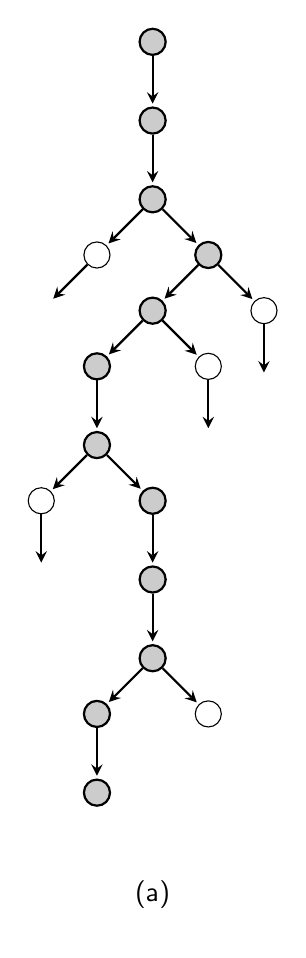
\begin{tikzpicture}[->,>=stealth,shorten >=1pt,auto,node distance=1cm,thick,main node/.style={fill=black!20,circle,draw,font=\sffamily}]
	
		\node[main node] (1) { };
		\node[main node] (2) [below of=1] { };
		\node[main node] (3) [below of=2] { };
		\node[main node, style={thin, fill=none}] (4) [below left of=3] { };
		\node[main node] (5) [below right of=3] { };
		\node[main node, style={draw=none, fill=none}] (erapraser6) [below left of=4] { };
		\node[main node] (6) [below left of=5] { };
		\node[main node, style={thin, fill=none}] (7) [below right of=5] { };
		\node[main node, style={thin, fill=none}] (8) [below right of=6] { };
		\node[main node] (9) [below left of=6] { };
		\node[main node, style={draw=none, fill=none}] (erapraser10) [below of=7] { };
		\node[main node, style={draw=none, fill=none}] (10) [below of=8] { };
		\node[main node] (11) [below of=9] { };
		\node[main node] (12) [below right of=11] { };
		\node[main node, style={thin, fill=none}] (13) [below left of=11] { };
		\node[main node] (14) [below of=12] { };
		\node[main node, style={draw=none, fill=none}] (15) [below of=13] { };
		\node[main node] (16) [below of=14] { };
		\node[main node] (17) [below left of=16] { };
		\node[main node, style={thin, fill=none}] (18) [below right of=16] { };
		\node[main node] (19) [below of=17] { };
		\node[main node, style={draw=none, fill=none}] (20) [below of=16] {};
		\node[main node, style={draw=none, fill=none}] (21) [below of=20] {};
		\node[main node, style={draw=none, fill=none}] (a) [below of=21] {(a)};
		
		\path[every node/.style={font=\sffamily\small}]
		(1) edge (2)
		(2) edge (3)
		(3) edge (4)
			edge (5)
		(4)	edge (erapraser6)
		(5) edge (6)
			edge (7)
		(6) edge (8)
			edge (9)
		(7) edge (erapraser10)
		(8) edge (10)
		(9) edge (11)
		(11)edge (12)
			edge (13)
		(12)edge (14)
		(13)edge (15)
		(14)edge (16)
		(16)edge (17)
			edge (18)
		(17)edge (19);
		
		\end{tikzpicture}
		
		%%%%%%%%%%%%%%%%%%%%%%%%%%%%%%%%%%%%%%%%%%%%%%%%%%%%%%%%%%%%%%%%%%
		

		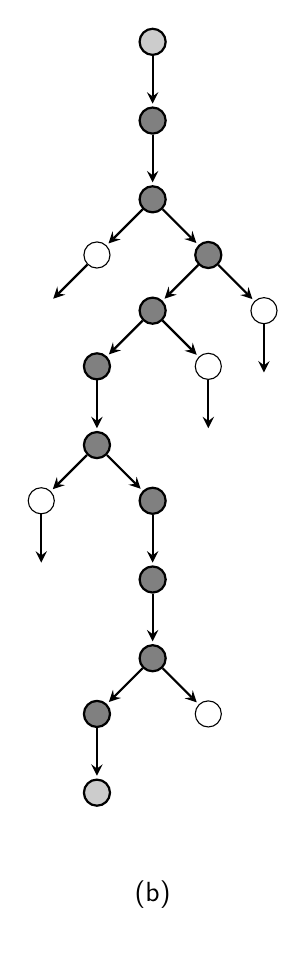
\begin{tikzpicture}[->,>=stealth,shorten >=1pt,auto,node distance=1cm,thick,main node/.style={fill=black!50,circle,draw,font=\sffamily}]
		
		\node[main node, style={fill=black!20}] (1) { };
		\node[main node] (2) [below of=1] { };
		\node[main node] (3) [below of=2] { };
		\node[main node, style={thin, fill=none}] (4) [below left of=3] { };
		\node[main node] (5) [below right of=3] { };
		\node[main node, style={draw=none, fill=none}] (erapraser6) [below left of=4] { };
		\node[main node] (6) [below left of=5] { };
		\node[main node, style={thin, fill=none}] (7) [below right of=5] { };
		\node[main node, style={thin, fill=none}] (8) [below right of=6] { };
		\node[main node] (9) [below left of=6] { };
		\node[main node, style={draw=none, fill=none}] (erapraser10) [below of=7] { };
		\node[main node, style={draw=none, fill=none}] (10) [below of=8] { };
		\node[main node] (11) [below of=9] { };
		\node[main node] (12) [below right of=11] { };
		\node[main node, style={thin, fill=none}] (13) [below left of=11] { };
		\node[main node] (14) [below of=12] { };
		\node[main node, style={draw=none, fill=none}] (15) [below of=13] { };
		\node[main node] (16) [below of=14] { };
		\node[main node] (17) [below left of=16] { };
		\node[main node, style={thin, fill=none}] (18) [below right of=16] { };
		\node[main node, style={fill=black!20}] (19) [below of=17] { };
		\node[main node, style={draw=none, fill=none}] (20) [below of=16] {};
		\node[main node, style={draw=none, fill=none}] (21) [below of=20] {};
		\node[main node, style={draw=none, fill=none}] (b) [below of=21] {(b)};
		
		\path[every node/.style={font=\sffamily\small}]
		(1) edge (2)
		(2) edge (3)
		(3) edge (4)
		edge (5)
		(4)	edge (erapraser6)
		(5) edge (6)
		edge (7)
		(6) edge (8)
		edge (9)
		(7) edge (erapraser10)
		(8) edge (10)
		(9) edge (11)
		(11)edge (12)
		edge (13)
		(12)edge (14)
		(13)edge (15)
		(14)edge (16)
		(16)edge (17)
		edge (18)
		(17)edge (19);
		
		\end{tikzpicture}
		
		%%%%%%%%%%%%%%%%%%%%%%%%%%%%%%%%%%%%%%%%%%%%%%%%%%%%%%%%%%%%%%%%%%
		
		
		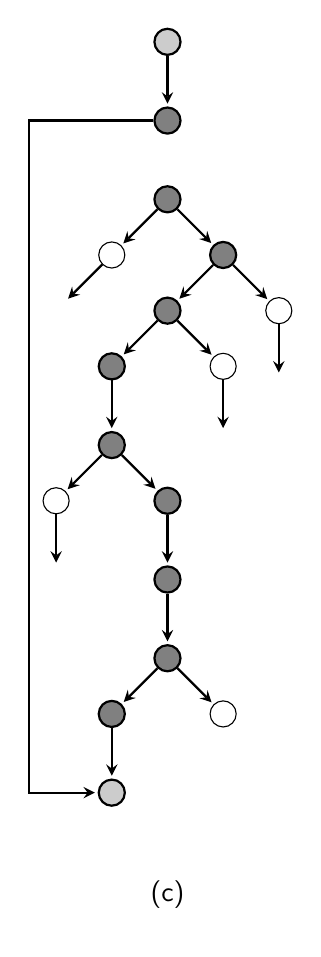
\begin{tikzpicture}[->,>=stealth,shorten >=1pt,auto,node distance=1cm,thick,main node/.style={fill=black!50,circle,draw,font=\sffamily}]
		
		\node[main node, style={fill=black!20}] (1) { };
		\node[main node] (2) [below of=1] { };
		\node[main node] (3) [below of=2] { };
		\node[main node, style={thin, fill=none}] (4) [below left of=3] { };
		\node[main node] (5) [below right of=3] { };
		\node[main node, style={draw=none, fill=none}] (erapraser6) [below left of=4] { };
		\node[main node] (6) [below left of=5] { };
		\node[main node, style={thin, fill=none}] (7) [below right of=5] { };
		\node[main node, style={thin, fill=none}] (8) [below right of=6] { };
		\node[main node] (9) [below left of=6] { };
		\node[main node, style={draw=none, fill=none}] (erapraser10) [below of=7] { };
		\node[main node, style={draw=none, fill=none}] (10) [below of=8] { };
		\node[main node] (11) [below of=9] { };
		\node[main node] (12) [below right of=11] { };
		\node[main node, style={thin, fill=none}] (13) [below left of=11] { };
		\node[main node] (14) [below of=12] { };
		\node[main node, style={draw=none, fill=none}] (15) [below of=13] { };
		\node[main node] (16) [below of=14] { };
		\node[main node] (17) [below left of=16] { };
		\node[main node, style={thin, fill=none}] (18) [below right of=16] { };
		\node[main node, style={fill=black!20}] (19) [below of=17] { };
		\node[main node, style={draw=none, fill=none}] (20) [below of=16] {};
		\node[main node, style={draw=none, fill=none}] (21) [below of=20] {};
		\node[main node, style={draw=none, fill=none}] (c) [below of=21] {(c)};
		
		\path[every node/.style={font=\sffamily\small}]
		(1) edge (2)
		%(2) edge (3)
		(3) edge (4)
		edge (5)
		(4)	edge (erapraser6)
		(5) edge (6)
		edge (7)
		(6) edge (8)
		edge (9)
		(7) edge (erapraser10)
		(8) edge (10)
		(9) edge (11)
		(11)edge (12)
		edge (13)
		(12)edge (14)
		(13)edge (15)
		(14)edge (16)
		(16)edge (17)
		edge (18)
		(17)edge (19);
		
	    \draw 
	    (2.west)
	    -- ++(left:4.5em) 
	    |- (19.west);
		
		\end{tikzpicture}
	\end{multicols}

\legend{Fonte: elaborada pelo autor}
\end{figure}

\subsection{Identificação e memorização de traces}
\label{Fundamentacao:DTM:Identificacao}

A primeira etapa do processo de DTM é a identificação de traces. Traces são conjuntos sequenciais de instruções válidas redundantes e que não possuem efeitos colaterais. Instruções são consideradas redundantes quando, dado um determinado conjunto de entradas, a instrução produzirá sempre o mesmo resultado. Exemplos de instruções redundantes e sem efeitos colaterais incluem instruções lógicas e aritméticas e de desvio condicional e incondicional. Instruções que manipulam a memória primária e que executam sub-rotinas do sistema não são redundantes e possuem efeitos colaterais, portanto não serão constituintes de um trace. No caso da arquitetura SPARC também foram consideradas não redundantes as instruções que manipulam as janelas de registradores, já que adicionaram uma complexidade muito grande à criação e armazenamento de traces.

Operações envolvendo ponto-flutuante possuem a mesma caracterização quanto à redundância e causalidade de efeitos colaterais que as instruções citadas acima. Por exemplo, instruções aritméticas com ponto-flutuante são redundantes enquanto a manipulação de memória envolvendo-os não. Porém, como \citeonline{gabbay1996speculative} observa, instruções de ponto flutuante costumam ter baixa localidade espacial, o que no caso da construção de uma unidade de DTM as torna indesejáveis, por adicionarem complexidade desnecessária tendo em vista o baixo retorno causado por sua inclusão. Isso não impede que a técnica de memorização seja empregada em operações de ponto-flutuante para aumentar seu desempenho, como demonstrado por \citeonline{citron1998accelerating}.

Após a identificação do trace, se dá o processo de memorização. A memorização consiste em armazenar as informações necessárias para permitir a identificação de uma oportunidade de reuso de um trace, além de garantir que o circuito seja capaz de gerar corretamente as saídas necessárias e realizar um desvio para a próxima instrução a ser executada.



\subsection{Reuso de traces}
\label{Fundamentacao:DTM:Reuso}

O reuso de um trace ocorre quando este é redundante e possui uma instância memorizada equivalente ao que deve ser executado. Essas instâncias são equivalentes quando possuem a mesma sequência de instruções e o mesmo contexto de entrada.

O contexto de entrada é definido como o conjunto de valores utilizados no trace cuja origem é externa ao trace. De forma análoga, o contexto de saída são os valores gerados internamente ao trace e que estão disponíveis para uso externo ao término deste.

Como exemplo, tomemos um trace para o pseudocódigo demonstrado na figura \ref{Fig:ExemploContexto1}. Em um trace gerado após a execução desse código, os valores contidos em $a$, $b$ e $c$ são utilizados internamente antes de terem seus valores definidos no próprio trace, compondo então o contexto de entrada.

\begin{figure}[!h]
	\label{Fig:ExemploContexto1}
	\caption[Exemplo de pseudocódigo]{
		Exemplo de pseudocódigo.}
	
		\begin{algorithmic}
			\STATE $c \leftarrow c + a$
			\STATE $x \leftarrow c + b$
			\IF{$x \le 5$}
			\STATE $y \leftarrow x * 2$
			\ELSE
			\STATE $x \leftarrow x + 1$
			\ENDIF
		\end{algorithmic}
	\legend{Fonte: elaborada pelo autor}
\end{figure}

Suponhamos os valores de entrada como $a = 1$, $b = 2$ e $c = 3$. Com esses valores as instruções armazenadas no trace resultante se assemelhariam com o trace representado na figura \ref{Fig:ExemploContexto2}\footnote{Estariam inclusas no trace também as instruções de comparação e desvio responsáveis pelo desvio condicional, mas por terem formato e efeitos relativos à arquitetura foram omitidas para maior clareza no exemplo.}. 
%. Estariam inclusas no trace também as instruções de comparação e desvio responsáveis pelo desvio condicional, mas por terem formato e efeitos relativos à arquitetura foram omitidas para maior clareza no exemplo.

\begin{figure}[!h]
	\label{Fig:ExemploContexto2}
	\caption[Exemplo de trace para o pseudocódigo da figura \ref{Fig:ExemploContexto1}]{
		Exemplo de trace para o pseudocódigo da figura \ref{Fig:ExemploContexto1}.}
	
	\begin{algorithmic}
		\STATE $c \leftarrow c + a$
		\STATE $x \leftarrow c + b$
		\STATE $x \leftarrow x + 1$
	\end{algorithmic}
	\legend{Fonte: elaborada pelo autor}
\end{figure}

Com os valores do contexto de entrada contidos no parágrafo anterior, o contexto de saída deste trace é $c = 4$ e $x = 7$. Assim, sempre que os valores do contexto de entrada se igualarem a esses ao entrar no trace, não há necessidade de execução das instruções, ocorrendo então a escrita do contexto de saída diretamente. Como essas instruções não possuem efeito colateral, esse processo é transparente para o programa sendo executado.

É possível então observar a importância da memorização correta do trace. Ainda analisando o pseudocódigo da figura \ref{Fig:ExemploContexto1}, caso o contexto de entrada seja $a = 1$, $b = 2$ e $c = 1$, o contexto de saída é $c = 2$, $x = 4$ e $y = 8$. O trace gerado para essa execução difere do trace descrito anteriormente, tanto nas instruções contidas como nos resultados gerados, de forma que o reuso do trace impróprio pode levar a aplicação que está executando a produzir resultados incorretos.

\section{DTM em hardware}
\label{Fundamentacao:DTMHardware}

Na seção \ref{Fundamentacao:DTM} é explanado o funcionamento da técnica DTM de forma abstrata, sem detalhar como implementar em hardware um mecanismo capaz de executar tal tarefa. Esta seção apresenta uma possível implementação, descrita por \citeonline{costa2001explorando}.

A implementação de \citeonline{costa2001explorando} tem como alvo um processador com ISA MIPS I, uma ISA do tipo RISC tal qual a ISA SPARC, se assemelhando em muitas características ao processador LEON3 utilizado neste trabalho. Assim, a implementação apresentada nesta seção é adaptada para se adequar à ISA e desenho do LEON3.

Para armazenamento das informações relevantes ao reuso de um trace será utilizada uma unidade de memória denominada \tablet. Essa unidade de memória será organizada como uma tabela, na qual cada linha corresponde a um trace armazenado. Também é utilizada uma tabela para o armazenamento de informações sobre instruções individuais, denominada \tableg. Esta será utilizada para o reuso de instruções isoladas, enquanto aquela para o reuso de blocos de instruções sequenciais.

\subsection{A unidade \tableg}
\label{Fundamentacao:DTMHardware:TableG}

Como descrito anteriormente, o primeiro passo do processo de DTM é a identificação de instruções redundantes. Para que o reuso dessas instruções possa ser feito é necessário que as instâncias executadas sejam armazenadas em alguma estrutura, de forma que quando for identificada a redundância o resultado prévio possa ser prontamente utilizado.

Para cumprir este papel, foi projetada uma unidade de memória para armazenar uma tabela, denominada \tableg. A \tableg\ tem como função armazenar instâncias anteriores e permitir a leitura de resultados. Para que esses valores possam ser lidos e gravados de forma eficiente, essa tabela foi projetada tendo em cada linha uma instância de uma instrução redundante e em cada coluna um campo que deve ser armazenado.

\begin{figure}
	\label{Fig:MemoTableG}
	\caption[Representação da tabela \tableg]{
		Representação da tabela \tableg.}
	\begin{center}
		%A famosa gambiarra ataca novamente
		\newcommand{\tabela}[1]{
			\multicolumn{1}{|c|}{$#1$}
		}
		\begin{tabular}{*{8}{c}}
			tamanho em bits & $32$ & $32$ & $32$ & $32$ & $1$ & $1$ & $1$ \\
			\cline{2-8}
			& \tabela{pc} & \tabela{sv1} & \tabela{sv2} & \tabela{res/targ} & \tabela{jmp} & \tabela{brc} & \tabela{btaken} \\
			\cline{2-8}
			& \multicolumn{7}{c}{\vdots} \\
			\cline{2-8}
			& \tabela{pc} & \tabela{sv1} & \tabela{sv2} & \tabela{res/targ} & \tabela{jmp} & \tabela{brc} & \tabela{btaken} \\
			\cline{2-8}
		\end{tabular}
	\end{center}
	\legend{Fonte: elaborada pelo autor}
\end{figure}

Na figura \ref{Fig:MemoTableG} pode ser vista a distribuição dos bits na \tableg. Abaixo é definido o significado dos valores a serem estocados em cada campo da tabela:

\begin{itemize}
	\item $pc$: Responsável por armazenar o valor do contador de programa quando a instrução foi executada. Esse valor nada mais é que o endereço de memória onde está localizada a instrução.
	\item $sv1$: Armazena o valor do primeiro parâmetro passado para a instrução.
	\item $sv2$: Armazena o valor do segundo parâmetro passado para a instrução.
	\item $res/targ$: Campo onde é salvo o resultado da computação realizada, seja o resultado de uma instrução lógica, aritmética ou o endereço para um desvio.
	\item $jmp$: Caso a instrução seja um desvio incondicional será setado em $1$. Caso contrário estará em $0$.
	\item $brc$: Caso a instrução seja um desvio condicional será setado em $1$. Caso contrário estará em $0$.
	\item $btaken$: Caso a instrução seja um desvio condicional e tenha sido tomado, será setado em $1$. Caso contrário, não tendo sido tomado, estará em $0$. Caso não seja um desvio condicional seu valor é indeterminado.
\end{itemize}

Colocando esses valores armazenados em \tableg\ no contexto da técnica DTM, o campo $pc$ é utilizado para identificar a qual instrução pertence aquela instância armazenada. Como é necessário o armazenamento do campo $pc$ para identificação, não há razão para armazenar a tabela de outra forma que não completamente associativa. Os valores de $sv1$ e $sv2$ compõe o contexto de entrada de uma única instrução, podendo esta fazer uso de apenas um ou ambos de acordo com seu formato. Em $res/targ$ temos o contexto de saída da instrução.

Os três campos de um bit servem para identificar como deve ser utilizado o resultado. Caso os três tenham valor $0$, $res/targ$ é copiado para o registrador de destino indicado na instrução. Caso $jmp$ seja $1$, o valor de $res/targ$ é somado ao registrador de programa, o PC, realizando assim um desvio incondicional. Caso $brc$ esteja ativo a instrução é um desvio condicional, e o valor de $res/targ$ é somado ao PC caso $btaken$ também esteja ativo. Independentemente do valor de $btaken$, caso $brc$ esteja ativo ambos os bits serão utilizados para atualizar a unidade de predição de desvios, caso este exista.

\subsection{A unidade \tablet}
\label{Fundamentacao:DTMHardware:TableT}

Analogamente à \tableg, a \tablet\ tem como objetivo armazenar dados de instâncias de instruções armazenadas afim de permitir o reuso destas em execuções futuras. Porém, diferentemente daquela, esta armazena informações sobre traces, sendo então responsável por guardar todas as informações necessárias para o reuso de um conjunto de duas ou mais instruções redundantes.

O projeto da \tablet, apesar de compartilhar características com a estrutura da \tableg, deve ser adaptado para que o armazenamento de informações sobre um trace completo possam ser utilizadas de forma a identificar um trace redundante e reutilizá-lo de forma transparente à aplicação utilizando a unidade de processamento. 

A \tablet\ é então também uma unidade de memória completamente associativa organizada em forma tabular na qual cada linha representa um trace, ou seja uma instância de execução de uma sequência de instruções, e cada coluna um campo necessário para identificação ou reuso correto deste trace. A descrição destes campos, que podem ser vistos na figura \ref{Fig:MemoTableT}, segue abaixo:

\begin{itemize}
	\item $pc$: Onde é guardado o endereço de memória da primeira instrução do trace, usado para identificação de candidatos a reuso.
	\item $npc$: Armazena o endereço de memória da próxima instrução a ser executada. Após o reuso de um trace é necessário um desvio para a instrução subsequente, sendo então utilizado o valor de $npc$ para o cálculo desse desvio.
	\item $icr$: Identifica quais registradores pertencem ao contexto de entrada.
	\item $icv$: Armazena os valores do contexto de entrada, contido nos registradores indicados pelo campo $icr$.
	\item $ocr$: Identifica quais registradores pertencem ao contexto de saída.
	\item $ocv$: Armazena os valores do contexto de saída, contido nos registradores indicados pelo campo $ocr$.
	\item $bmask$: Máscara na qual cada bit em nível alto indica a presença de um desvio no trace.
	\item $btaken$: Máscara que armazena para cada desvio indicado em $bmask$ se ele foi tomado ou não.
\end{itemize}

\begin{figure}
	\label{Fig:MemoTableT}
	\caption[Representação da tabela \tablet]{
		Representação da tabela \tablet.}
	\begin{center}
		%A famosa gambiarra ataca novamente novamente
		\newcommand{\tabela}[1]{
			\multicolumn{1}{|@{ }c@{ }|}{#1}
		}
		
		\newcommand{\tabelatripla}[2]{
			\tabela{$#1_{1}$} & \tabela{\hdots} & \tabela{$#1_{#2}$}
		}
		
		\tiny
%		\begin{tabular}{*{21}{c}}
%			tamanho em bits & $32$ & $32$ & \multicolumn{3}{c}{$5 * N_{1}$} & \multicolumn{3}{c}{$32 * N_{1}$} & \multicolumn{3}{c}{$5 * N_{2}$} & \multicolumn{3}{c}{$32 * N_{2}$} & \multicolumn{3}{c}{$1 * B$} & \multicolumn{3}{c}{$1 * B$} \\
%			\cline{2-21}
%			& \tabela{$pc$} & \tabela{$npc$} & \tabelatripla{icr}{N_{1}} & \tabelatripla{icv}{N_{1}} & \tabelatripla{ocr}{N_{2}} & \tabelatripla{ocv}{N_{2}} & \tabelatripla{bmask}{B} & \tabelatripla{btaken}{B}  \\
%			\cline{2-21}
%			\multicolumn{21}{c}{\vdots} \\
%			\cline{2-21}
%			& \tabela{$pc$} & \tabela{$npc$} & \tabelatripla{icr}{N_{1}} & \tabelatripla{icv}{N_{1}} & \tabelatripla{ocr}{N_{2}} & \tabelatripla{ocv}{N_{2}} & \tabelatripla{bmask}{B} & \tabelatripla{btaken}{B}  \\
%			\cline{2-21}
%		\end{tabular}
		\normalsize
		
	\end{center}
	\legend{Fonte: elaborada pelo autor}
\end{figure}

A figura \ref{Fig:MemoTableT} também indica o uso de três parâmetros configuráveis: $N_{1}, N_{2}, B  \in \mathbb{Z}$. O significado de cada um é explicado a seguir.

$N_{1}$ define quantos registradores podem pertencer ao contexto de entrada de um trace. Caso o para continuar a construção do trace esse seja necessário mais registradores, a construção será encerrada. 

Com uso bastante semelhante a $N_{1}$, $N_{2}$ limita a quantidade de registradores no contexto de saída. \citeonline{costa2001explorando} utiliza $N_{1}, N_{2} \mid N_{1} = N_{2}$, mas isso não é necessário para o funcionamento correto do DTM. Em aplicações que os traces comumente possuem mais valores no contexto de saída que no de entrada é desejável criar a tabela tal que $N_{1} < N_{2}$. Da mesma forma, caso o contexto de entrada costume ser maior que o de saída, podem ser escolhidos valores para os quais $N_{1} > N_{2}$. Cabe ao projetista ajustar a unidade para melhor se adaptar as características dos traces nela armazenados, atingindo assim melhor desempenho e evitando desperdício de memória.

Por fim, $B$ indica a quantidade máxima de instruções de desvio que serão armazenadas em um trace. Os valores armazenados em $bmask$ e $btaken$ são utilizados para atualizar as unidades de predição de desvio. Caso a aplicação envolva muitas instruções de desvio, aumentar o valor de $B$ aumentará o tamanho máximo dos traces armazenados, permitindo o reuso de mais instruções com uma única entrada.

Esses parâmetros devem ser definidos no momento da construção do hardware. A existência desses se deve ao fato de não interferirem no bom funcionamento da técnica mas influenciar os resultados. A medida que se aumenta o valor dos parâmetros o tamanho máximo dos traces também aumenta, o que pode causar um ganho de desempenho dependendo da aplicação sendo executada. Porém, esses valores são diretamente proporcionais à quantidade de memória necessária para o armazenamento, aumentando a área de chip e o custo do hardware resultante.


\subsection{Construção e reuso}
\label{Fundamentacao:DTMHardware:Integracao}

Para construção de um trace são utilizados dois mapas de contexto e um \textit{buffer} temporário. Esse \textit{buffer} possui o mesmo formato de uma linha da \tablet, enquanto os mapas possuem um bit para cada registrador, totalizando 32 bits.

Quando uma instrução redundante é identificada se inicia a construção do trace. O valor do registrador PC é inserido no \textit{buffer} no campo $pc$, enquanto seu valor somado 4 no $npc$. Para cada registrador pertencente ao contexto de entrada, o respectivo bit na máscara de contexto de entrada é posta em nível alto. Caso o bit estivesse em $0$, o número do registrador e seu valor são inseridos no \textit{buffer}. O mesmo se aplica ao mapa de contexto de saída, com a diferença que caso haja duas escritas em um registrador o valor em $ocv$ é atualizado, o que não ocorre no contexto de entrada. Caso a instrução a ser executada seja um desvio, os devidos bits são escritos nas máscaras do \textit{buffer} temporário. 

Para cada instrução subsequente, caso seja redundante, o campo $npc$ recebe o valor do registrador PC mais quatro, enquanto os outros valores são inseridos e atualizados como descrito anteriormente. Caso a instrução não seja redundante o \textit{buffer} é escrito em uma entrada da \tablet\ e os valores do \textit{buffer} e dos mapas são zerados.

Paralelamente, para cada instrução é verificado em \tableg\ e \tablet\ se existem entradas para as quais valor de $pc$ equivale ao do registrador PC. Para as que são encontradas, é verificado então o contexto de entrada. Os registradores indicados pelo campo $icr$ tem seus valores lidos do banco de registradores e comparados com os valores de $icv$ para cada entrada identificadas de \tablet. Já para \tableg, os registradores indicados na própria instrução tem seus valores comparados com os campos $sv1$ e $sv2$. Caso haja um trace em \tablet\ no qual todos os registradores passem neste teste, ele então é reusado. Caso não haja um trace mas haja um instrução em \tableg, ela então é reusada. Caso contrário, a instrução é executada normalmente.

\section{O LEON3}
\label{Fundamentacao:LEON3}

O LEON3 é um processador 32-bit baseado na arquitetura SPARC V8 atualmente mantido pela Cobham Gaisler. Disponibilizado sob a licensa GPL, o código-fonte é na linguagem VHDL e implementado utilizando \textit{generics}, o que permite a configuração dos parâmetros que definem algumas características do processador \cite{grlibmanual}.

O LEON3 possui um banco de registradores com suporte para 2 a 32 janelas. Cada janela tem acesso a 32 registradores:

\begin{itemize}
	\item \textit{Global}: 8 registradores acessíveis por todas as janela. Utilizados para armazenamento de valores globais. Registradores 0 a 7.
	\item \textit{Out}: 8 registradores acessíveis pela janela atual e pela próxima janela. Utilizados para passagem de parâmetros e recebimento de valores de retorno. Registradores 8 a 15.
	\item \textit{Local}: 8 registradores acessíveis somente pela janela atual. Utilizados para variáveis locais e valores temporários. Registradores 16 a 23.
	\item \textit{In}: 8 registradores acessíveis pela janela atual e pela janela anterior. Utilizados para recebimento de parâmetros e retorno de valores. Registradores 24 a 31.
\end{itemize}

A janela atual é determinada pelo \textit{Current Window Pointer}, um contador de 5 bits contido no registrador \textit{Processor State Register}. O contador é incrementado com a instrução RETT e decrementado com a SAVE. O objetivo dessas janelas é agilizar a troca de contexto, permitindo a mudança de vários registradores para um valor anterior em menos instruções \cite{sparcmanual}.

\begin{figure}
	\label{Fig:Leon3Interno}
	\caption[Diagrama de blocos interno do LEON3]{
		Diagrama de blocos interno do LEON3.}
	\begin{center}
		\includegraphics[width=\linewidth]{fig/leon3interno.pdf}
	\end{center}
	\legend{Fonte: \cite{leondatasheet}}
\end{figure}

Ao configurar o sistema antes da compilação do código-fonte também é possível optar pela inclusão de uma unidade de processamento de ponto-flutuante. Duas unidades estão disponíveis, a GRFPU e a GRFPU-Lite, ambas se adequando ao padrão IEEE-754.

Além dessas unidades, como demonstrado na figura \ref{Fig:Leon3Interno} são incluídas outras unidades como suporte a depuração, multiplicadores e divisores em hardware, entre outros \cite{grlibmanual}.


\begin{figure}
	\label{Fig:Leon3Externo}
	\caption[Diagrama de blocos de um sistema utilizando o GRLIB]{
		Diagrama de blocos de um sistema utilizando o GRLIB.}
	\begin{center}
		\includegraphics[width=\linewidth]{fig/leon3externo.pdf}
	\end{center}
	\legend{Fonte: \cite{grlibmanual}}
\end{figure}

A unidade de inteiros, que lida com as instruções que não são de ponto-flutuante na arquitetura SPARC, é organizada em um pipeline de 7 estágios:

\begin{enumerate}
	\item FE (\textit{Instruction Fetch}): A instrução é buscada na cache de instruções. Caso haja um \textit{miss} a devida instrução é buscada no barramento.
	\item DE (\textit{Decode}): A instrução é decodificada. O endereço de desvio é calculado.
	\item RA (\textit{Register Access}): Os registradores utilizados são lidos do banco ou de alguma unidade de \textit{fowarding}.
	\item EX (\textit{Execute}): Operações lógicas e aritméticas são executadas. Endereços de acesso de memória e de retorno de chamada são calculados.
	\item ME (\textit{Memory}): Caso a instrução requisite, é feito um acesso à cache de dados. Na ocorrência de um \textit{miss} ou de uma escrita (o tratamento de escritas é \textit{write-through}) o comando é enviado ao barramento principal.
	\item XC (\textit{Exception}): Tratamento de excessões e interrupções.
	\item WR (\textit{Write}): O resultado da operação lógica ou aritmética é escrito no banco de registradores.
\end{enumerate}

As memórias caches são separadas para instruções e dados. Seus tamanhos, formatos e associatividades são configuráveis. A presença de uma MMU para auxiliar o gerenciamento de memória é opcional. As requisições de memória são realizadas para o barramento AHB.

Como pode ser visto na figura \ref{Fig:Leon3Externo}, um sistema GRLIB utiliza uma barramento segundo o padrão AMBA 2.0. O processador é conectado ao barramento AHB, juntamente com o controlador de memória e outras unidades como entradas para JTAG, USB, Ethernet, entre outros. Também está conectado neste barramento um controlador ponte para o APB. O APB é responsável por controle dos periféricos, como temporizadores e portas de entrada e saída de dados  \cite{grlibmanual}.


\section{FPGA}
\label{Fundamentacao:FPGA}

Devido a sua versatilidade e relativo baixo custo, decidiu-se por utilizar a tecnologia de FPGA para realização dos testes de hardware. Para produção de poucas unidades, tecnologias ASIC possuem um custo por unidade muito maior que o uso de FPGA, além desta oferecer a possibilidade de realização de modificações no hardware depois de pronto, o que é impossível naquela \cite{chu2006rtl}.

Nesta seção será apresentado brevemente o funcionamento de um circuito de FPGA. A intenção é permitir ao leitor a compreensão que mesmo sendo diferente de um circuito impresso, um circuito gravado em FPGA compartilhará de quase todas as suas características apesar de sua diferente configuração.

%%%%%%%%%%%%%%%%%%%%%%%%%%%%%%%%%%%%%%%%%%%%%
%%%% <REESCREVER>

Como dito anteriormente, chips de FPGA são programáveis e, apesar de serem mais caros que um CI de produção em massa, é muito mais barato para poucas unidades a gravação em FPGA que a criação de um CI específico. Porém, apesar de se mostrarem mais lentos que circuitos usando tecnologias ASIC, os circuitos em FPGA possuem um comportamento semelhante a suas a estes, já que placas de FPGA foram feitas para emularem as conexões entre elementos lógicos contidas em um circuito ASIC.
Isso os torna ideais para prototipação e testes de hardware, já que é possível testar de forma barata e versátil a funcionalidade e características de um determinado circuito. 

Além disso, a comparação de modelos gravados em circuito utilizando uma tecnologia como FPGA permite tirar conclusões para esses modelos, mesmo que sejam utilizados posteriormente de outras maneiras. Cabe ressaltar que a comparação de valores entre projetos de circuito deve considerar a proporcionalidade causada pela diferença de tecnologias \cite{tanenbaum2009organizacao}.

%%%% </REESCREVER>
%%%%%%%%%%%%%%%%%%%%%%%%%%%%%%%%%%%%%%%%%%%%%

Um circuito de FPGA é composto principalmente de \textit{Lookup Tables} e interconexões programáveis. A replicação desses componentes e a possibilidade de programá-los independentemente dá ao FPGA uma capacidade de criar diversos circuitos lógicos de acordo com os valores dados.

Uma LUT é uma pequena unidade de memória que armazena valores determinados pelo hardware a ser gerado. Ao combinar os pinos de endereçamento formando uma posição de memória, o valor gravado é lido e colocado nos pinos de saída. Dessa forma uma LUT é capaz de simular o funcionamento de qualquer função lógica que possua um número de entradas menor ou igual seu número de pinos de endereçamento. Combinando as entradas e saídas de unidades que contém uma LUT de forma programável permite a emulação de uma infinidade de circuitos lógicos, limitados apenas pela quantidade de elementos lógicos contidos no chip utilizado \cite{tanenbaum2009organizacao}.

Neste trabalho foi feito uso do dispositivo Altera Cyclone II. Neste as LUT possuem 16 posições de memória, com quatro pinos para endereçamento. Essas LUT estão contidas em unidades chamadas \textit{Logic Elements}, que são a unidade lógica mínima na arquitetura. Uma LE também possui um registrador programável e suporte para sinal de \textit{feedback}, \textit{clock} e \textit{clear}. Por estarem agrupadas em conjuntos denominados \textit{Logic Array Blocks}, cada LE possui um sinal de entrada \textit{carry in} e um sinal de saída \textit{carry out}, facilitando o uso de conjuntos de LE para operações aritméticas \cite{altera2007cyclone}.
%
%\chapter{Desenvolvimento e implementação}
%\label{Desenvolvimento}
%\input{desenvolvimento.tex}
%
%\chapter{Análise dos resultados}
%\label{Analise}
%\input{analise.tex}



% ---
% Finaliza a parte no bookmark do PDF, para que se inicie o bookmark na raiz
% ---
\bookmarksetup{startatroot}% 
% ---

% ---
% Conclusão
% ---
%\chapter[Conclusão]{Conclusão}
%\label{Conclusao}
%%%\chapter{Conclusão} - manter comentado
%
%	\begin{flushright}
%		\textit{``As palavras fogem quando precisamos delas e 
%		\\sobram quando não pretendemos usá-las.''\\Carlos Drummond de Andrade}
%	\end{flushright}
%
%%\textbf{Justificativa e objetivo da tese.}
%Esta pesquisa justifica-se pela necessidade de se implementar sistemas automáticos de recuperação de informação que deem suporte adequado à informação corporativa e às tarefas dos usuários corporativos. Para isso, se buscou uma compreensão mais geral da informação corporativa que beneficie sua evolução contínua e não a limite a um cenário de uso excessivamente reduzido. Para isso, foi realizada uma análise do domínio corporativo com o objetivo de propor um conjunto de características da informação corporativa.
%
%%\textbf{Resultados obtidos.}
%Assim, este trabalho empreendeu uma análise preliminar de domínio pela aplicação da técnica de análise facetada sobre informação corporativa. Foram identificadas características potencialmente comuns às coleções; e um protótipo de sistema de recuperação de informação corporativa e um conjunto de expressões de busca de usuários reais serviram para avaliar empiricamente e validar essas características identificadas.
%
%%Para responder ao problema proposto, o objetivo geral deste trabalho será propor um conjunto de características da informação corporativa que favoreça a organização e a recuperação da informação.
%%	\item Propor um conjunto de facetas que seja útil na organização automática da informação corporativa e na interoperabilidade entre diferentes repositórios de informação da mesma empresa ou de diferentes empresas;
%%	\item Identificar as facetas pelas quais os usuários de informação especificam sua necessidade de informação no contexto de trabalho;
%%	\item Avaliar as implicações da organização facetada da informação corporativa no desempenho dos sistemas automáticos de recuperação de informação.
%
%
%%\textbf{Sumário para próximas seções.}
%A seção \ref{conclusao-resultados} apresenta os principais resultados alcançados, enquanto a seção \ref{conclusao-limitacoes} apresenta discussões e limitações da pesquisa. Finalmente, a seção \ref{conclusao-futuros} aponta algumas direções para trabalhos futuros.
%
%
%
%
%\section{Resultados}
%\label{conclusao-resultados}
%
%%\textbf{3 resultados obtidos.}
%Três resultados foram obtidos neste trabalho. O primeiro resultado refere-se a um conjunto com 12 categorias que, como uma potencial representação da informação corporativa, pode servir como um modelo conceitual de longo prazo do domínio corporativo. O conjunto de categorias descobertas deve requerer revisões menos frequentes e suportar o desenvolvimento incremental de sistemas de recuperação de informação corporativa mais flexíveis e interoperáveis. O segundo resultado refere-se a um subconjunto das 12 categorias que é mobilizado especialmente por usuários no momento de elaborar expressões de busca com o objetivo de recuperar documentos de interesse.
%O terceiro resultado refere-se à validação de ambas as coleções corporativas como pertinentes para desenvolver e avaliar sistemas de recuperação de informação corporativa.
%
%%1
%%\textbf{1o resultado - 12 categorias.}
%O primeiro resultado teve sua origem na análise facetada empreendida sobre os dois exemplares do domínio corporativo. Ele corresponde à identificação de 12 categorias comuns às duas coleções corporativas. A distribuição de assuntos de ambas as empresas dentro das categorias apresentou alta correlação positiva. Isso sugere que autores e leitores, de ambas as empresas, embora necessitem de assuntos diferentes, mobilizam assuntos das mesmas categorias e facetas.
%%isso tem o potencial de melhorar o desempenho da indexação e recuperação automática de informação corporativa, na medida em que métodos especiais assumem a função de indexar, recuperar e ordenar as diferentes categorias e facetas.
%
%%\textbf{Facetas e subfacetas.}
%Além das categorias identificadas, foram também avaliadas as facetas e subfacetas. Embora úteis para cada coleção, a distribuição de assuntos em facetas e subfacetas entre as coleções não apresenta indício de correlação. Isso sugere que características exclusivas de algumas empresas requerem facetas e subfacetas especiais que favorecem a comunicação de seus atores sociais. O volume de atores sociais contidos na empresa, a extensão geográfica atendida por seus serviços e produtos, as atividades e o setor econômico são exemplos de características exclusivas que parecem interferir na composição das mensagens corporativas.
%
%%\textbf{Aumento do desempenho do SRI.}
%Em avaliação, as categorias não figuraram entre as fontes de evidência mais comuns dos experimentos apresentados na trilha \textit{Enterprise} da \textit{Text Retrieval Conference}. Entretanto, a simples implementação de um protótipo que considerou parte das categorias aumentou o desempenho do recuperação de informação. O aumento do desempenho ocorreu mesmo sem fazer uso de repositórios externos à empresa e sem o suporte de metabuscadores, algumas das estratégias adotadas em outros trabalhos. Comparando os resultados atuais com aqueles encontrados na literatura, facetas espaciais e temporais mostraram-se especialmente úteis, uma vez que quase não têm sido exploradas em trabalhos interpretativos e constituíram as fontes de evidência com maior potencial de contribuição para a recuperação e o \textit{ranking} da informação corporativa.
%
%%2
%
%%\textbf{2o resultado - 8 categorias.}
%O segundo resultado teve sua origem na análise facetada empreendida sobre as expressões de busca de usuários da coleção particular. As expressões de busca foram elaboradas com o objetivo de recuperar documentos previamente apresentados pelo usuário. Assim, o método serviu para investigar quais categorias e facetas eram reconhecidas no documento e mobilizadas pelo usuário enquanto usavam um sistema de recuperação de informação hipotético. A distribuição de assuntos em oito categorias, compatível com a distribuição de assuntos naquelas categorias descobertas no domínio, evidencia que os usuários mobilizam as categorias corretas para elaborar as expressões de busca.
%
%%\textbf{Evidência de que usuários da coleção pública não sabem escolher termos espaciais e temporais com a precisão correta.}
%Por outro lado, o experimento sobre a coleção pública evidenciou que os usuários da coleção pública, apesar de também mobilizarem as categorias corretas, não conseguem escolher corretamente os termos espaciais e temporais. Isso pode ser explicado pelo desconhecimento da precisão geográfica e temporal com a qual o documento foi produzido e indexado. No entanto, o primeiro resultado, discutido anteriormente, foi suficiente para compatibilizar a granularidade espacial e temporal de indexação e de recuperação.
%
%
%%3
%
%%\textbf{3o resultado - validação das coleções.}
%O terceiro resultado corresponde à validação cruzada da coleção de referência e da coleção particular. Coleções de referência usadas para avaliação de Cranfield normalmente são alvos de críticas sobre sua utilidade limitada para o desenvolvimento científico. Essa dificuldade também se apresenta para a coleção de referência adotada neste trabalho. Para enfrentar essa dificuldade, foi adotada também uma coleção particular. Uma vez que a coleção particular foi produzida por seus próprios usuários para ser usada no contexto de trabalho e tomada de decisão, ela pode ser vista como uma coleção suficiente para empreender novos estudos sobre informação corporativa. Por outro lado, a compatibilidade entre a distribuição de assuntos entre as categorias, facetas e subfacetas de ambas as coleções faz com que a coleção pública igualmente possa ser vista como uma coleção válida para estudos sobre informação corporativa.
%
%%\textbf{Coleção de avaliação adicional, em língua portuguesa.}
%Adicionalmente, uma vez que não havia qualquer iniciativa de construção de coleção de documentos corporativos em língua portuguesa, a coleção particular constitui um produto útil para trabalhos futuros. Porém, a aplicação da nova coleção difere da aplicação da coleção de referência, sendo mais apropriada para estudos interpretativos e históricos. A coleção da CSIRO, principalmente por seu tamanho e método de criação, é mais adequada para estudos empíricos baseados em métodos estatísticos e carece de uma maior diversidade de informação no escopo intraorganizacional.
%
%
%\section{Considerações e limitações}
%\label{conclusao-limitacoes}
%
%%12 facetas
%
%%\textbf{Apenas 2 empresas, poucos documentos, de pequena diversidade.}
%O número reduzido de empresas e coleções estudadas apresenta limitações para uma análise mais aprofundada e para uma generalização do domínio corporativo. Na coleção de referência pública, os documentos são de um conjunto muito restritivo, apenas da \textit{Web} pública da empresa, com necessidades de informação que poderiam ser atendidas pelo próprio cliente da empresa, através de um bom sistema de busca da \textit{Web}. Na segunda coleção, particular, há um número bem menor de documentos, porém com uma maior diversidade temporal e de atividades. Em nenhuma das coleções há exaustividade, o que nos remete à impossibilidade de representar todo e qualquer fenômeno do domínio, embora provavelmente representem os fenômenos mais comuns de ambas as empresas.
%
%%\textbf{Importância das características locais ou exclusivas.}
%Por outro lado, mesmo se for possível alguma generalização sobre as características do domínio corporativo, ela certamente não representa isoladamente toda a comunicação da qual as empresas precisam para realizar trabalho. Com isso, as características locais ou exclusivas de cada empresa continuam a desempenhar um papel importante na compreensão da comunicação dos seus diversos atores sociais.
%
%%\textbf{Características seriam suficientes para melhorar o desempenho do SRI.}
%Ao mesmo tempo, todas as características identificadas, das mais gerais até as mais específicas, parecem suportar a melhoria do desempenho de um sistema de recuperação de informação corporativa. Porém, as características mais específicas tendem a ser úteis apenas no contexto particular de uma organização, enquanto as características mais gerais provavelmente contribuem para empresas de todo o domínio corporativo.%isso aqui é resultado, não?
%
%%\textbf{Foram usadas apenas as categorias na avaliação empírica da coleção pública.}
%A recuperação de informação da coleção pública foi avaliada empiricamente utilizando-se apenas das características mais gerais (as categorias). Essa avaliação, tratada no capítulo \ref{prototipo}, embora destaque o valor das características comuns a ambas as empresas, requer cautela. De fato, não é possível generalizar o domínio corporativo a partir das duas empresas pesquisadas, assim como não é possível deduzir que todo o arquivo das empresas possui as mesmas características. A linguagem corporativa, como fenômeno social, está sujeita a um desenvolvimento contínuo e dinâmico, adaptando-se às necessidades das instituições e de seus atores sociais. Acompanhar continuamente essas mudanças parece ser a única saída para manter sistemas de recuperação de informação corporativa eficazes ao longo do tempo, adaptando-os para novas realidades de comunicação que são construídas ao longo do tempo.
%
%%\textbf{Há limitações na documentação da coleção pública.}
%Adicionalmente, a classificação de relevância de documentos para cada tarefa de busca da coleção pública não é bem documentada. Como a qualidade dessa classificação não pode ser atestada neste trabalho, os resultados do \textit{ranking} podem ser piores ou melhores que aqueles aferidos em outros trabalhos. 
%
%%Aumento do desempenho suporta a hipótese de que facetas diferentes são úteis para qualquer empresa. Na literatura há menor frequência de trabalhos sobre facetas sociais, espaciais e temporais.
%
%%O fenômeno social depende do tempo e da evolução concorrente das áreas do conhecimento que colaboram dentro das organizações.
%
%%Também depende de outras variáveis que afetam uma ou mais facetas, como espaço e redes sociais.
%
%%\textbf{Relevância não foi avaliada na coleção particular.}
%Relevância também não foi objeto de avaliação na coleção particular. A compatibilidade entre as expressões de busca e os documentos da coleção particular representa a uniformidade da comunicação corporativa, especificada tanto nos documentos quanto nas expressões de busca dos seus usuários, ao invés de provável relevância de documentos. A uniformidade da comunicação pode contribuir para recuperar e ordenar documentos baseando-se na sua utilidade para o contexto de trabalho. Para isso, é preciso explorar métodos mais adequados para quantificar e avaliar sua utilidade, percepção incompatível com aquela de relevância.% embora mesmo a noção de relevância não seja unânime e não possa facilmente ser formalizada.
%
%%\textbf{Avanços sobre coleções é menos importante que avanços sobre facetas.}
%Resultados empíricos de outras trilhas da \textit{Text Retrieval Conference} têm indicado que avanços tecnológicos sobre coleções influenciam menos o desempenho dos sistemas de recuperação de informação que avanços tecnológicos sobre facetas específicas. Como um exemplo, avanços em técnicas de identificação, desambiguação e recuperação de facetas sociais no domínio corporativo parecem repercutir positivamente em vários contextos ou várias coleções do domínio. Por outro lado, avanços na compreensão e no desempenho de uma coleção de uma só empresa, mesmo que contribua para o desempenho de um sistema de recuperação de informação aplicado àquela coleção, não contribui para o desempenho do mesmo sistema para qualquer outra empresa.
%
%%\textbf{Avanços sobre facetas não garantem aumento de desempenho em todo e qualquer domínio.}
%Porém, é preciso esclarecer que aperfeiçoamentos baseados em uma faceta do domínio corporativo, e.g. faceta social, não implica no mesmo ganho de desempenho em outros domínios. Portanto, é preciso garantir que sejam realizados estudos sobre facetas e domínios específicos, sem esperar que sistemas de recuperação de informação adequados para um domínio também sejam adequados para outros domínios aparentemente semelhantes. Isso justifica trabalhos futuros, usando as mesmas coleções e usando coleções corporativas adicionais, o que enfrenta a dificuldade permanente de construir coleções de documentos que sejam válidas sem que comprometam o sigilo de alguns dados corporativos.
%
%%\textbf{Comparação de coleções por meio de categorias, facetas e subfacetas mostrou-se útil.}
%Por outro lado, o método de comparação através de categorias, facetas e subfacetas mostrou-se valioso por conta da baixa exposição de dados e da alta comparabilidade, podendo servir a coleções diferentes e a diferentes pesquisadores. A técnica de análise facetada mostrou-se útil para descobrir características e comparar organizações sem expor em excesso seus ativos de informação, garantindo uma comparação simples e direta das categorias, facetas e subfacetas que constituem sua informação corporativa. Esse uso da análise facetada não foi observado na literatura. Adicionalmente, a classificação facetada resultante, além de útil para trabalhos futuros sobre informação corporativa, constitui um exemplar de classificação facetada construído fora da biblioteca e para fins não-didáticos. Esse último produto contribui para aperfeiçoar os guias metodológicos e estudos empíricos acerca da própria técnica de análise facetada \cite{wild2009describing,labarre2010}.
%
%
%
%%validação da coleção
%
%
%%The work uses only two enterprise collections and more repositories are needed to evaluate the compatibility of terminology and the meaningful of the proposed facets for the whole enterprise domain. Both the companies are in the quaternary economic sector (i.e. education; and research and development). Studies about companies in other economic sectors are very important, since the knowledge and information can assume different roles and different behaviour. Additionally, the difficulties of accessing to enterprise repositories is a permanent issue. However, one can compare enterprise repositories by applying the facet analysis and by comparing the subjects rather than the  data. 
%
%
%%Não é possível generalizar
%
%
%%Mesmo facetas e subfacetas são úteis para aumentar desempenho de SRIC, mas localmente, ou seja, atende só a uma organização e não várias do domínio.
%
%%O empírico
%
%
%
%
%
%\section{Trabalhos futuros}
%\label{conclusao-futuros}
%
%%\textbf{Sumário para próximos parágrafos.}
%Os resultados deste trabalho sugerem algumas direções promissoras de trabalho futuro: a exploração de coleções corporativas adicionais; a exploração mais aprofundada de características da informação corporativa; novos estudos sobre o uso e o desempenho de sistemas de recuperação de informação; e o estudo de indexação automática da informação facetada.
%
%%-
%
%%\textbf{trabalho futuro 1.}
%Os resultados demonstram que as empresas apresentam muitas semelhanças e também muitas diferenças entre si. Portanto, a criação de mais coleções de referência é uma necessidade permanente. É preciso reunir amostras de dados de um número maior de organizações, com características que sejam úteis para trabalhos futuros, sem que as pesquisas se desenvolvam sobre apenas uma ou algumas poucas coleções de referência. Ao mesmo tempo em que novas coleções surgem, é importante que versões atualizadas também sejam produzidas de modo a permitir uma avaliação mais histórica do desenvolvimento da documentação, da linguagem corporativa e das necessidades dos usuários de uma dada organização. 
%
%%\textbf{trabalho futuro 1 - explicação.}
%Apenas dessa forma, se pode alcançar uma representação mais generalista do domínio ou pode ser identificada a impossibilidade de alcançá-la. Embora essa necessidade seja sugerida neste trabalho, reunir tantas empresas com dados abertos não é tarefa trivial. Uma solução intermediária passa pela caracterização da informação de várias empresas sem que os dados sejam livremente expostos. A análise de assuntos e a análise facetada atendem esses requisitos.
%
%%-
%
%%\textbf{trabalho futuro 2.}
%Também é importante diversificar as atividades e setores econômicos. Além disso, dentro do domínio corporativo, é preciso identificar as especificidades que idiomas, setores econômicos, atividades econômicas, tamanho da rede social corporativa, tipos de documentos e gêneros textuais provocam na informação corporativa.
%
%%\textbf{trabalho futuro 2 - explicação complementar.}
%A análise preliminar de domínio apontou que as facetas e subfacetas descobertas acomodam assuntos que são específicos de determinados contextos de uso. É o caso de facetas e subfacetas de elevada precisão geográfica, dentro da categoria Espaço. Em empresas com escopo geográfico urbano, são comuns os nomes de bairro, nomes de cidades vizinhas, nomes de capitais de estados vizinhos e nomes de empresas que correspondam a referências geográficas (agências bancárias, supermercados, hospitais, dentro outras). Ao contrário, em empresas com escopo geográfico nacional, são incomuns essas referências e tornam-se mais comuns os nomes de estados, nomes de cidades, nomes de empresas que não correspondem a referências geográficas (grandes empresas e multinacionais), e nomes de países.
%
%
%
%%-
%
%%\textbf{trabalho futuro 3 - novos modelos de interação.}
%Na perspectiva do uso da informação, é preciso estudar e experimentar novos modelos de interação que se beneficiem da classificação facetada da informação, além da busca por palavras-chaves. É o caso da navegação facetada, por exemplo, que passa a ser possível e mostra-se mais flexível para atender a uma maior diversidade de contextos de uso e necessidades de informação. Também é preciso experimentar novos modelos de ordenação de resultados (\textit{ranking}) que permita um ajuste fino e personalizado de facetas potencialmente mais úteis para certos grupos de usuários. Nesses casos, é preciso realizar estudos sobre estruturas de dados específicas para informação facetada e o seu papel no desempenho e na eficácia de sistemas de recuperação de informação.
%
%%\textbf{trabalho futuro 3 - comparação de desempenho entre organização da informação facetada e outras abordagens.}
%Na avaliação do impacto da organização facetada na eficiência da recuperação e no \textit{ranking} da informação corporativa, deve-se compará-la ao desempenho obtido através das estratégias de vocabulário controlado, de dados ligados externos (\textit{linked data}), de busca em texto completo, dentre outras.
%
%%\textbf{trabalho futuro 3 - representação de grandes massas de dados.}
%Adicionalmente, aplicações que têm se beneficiado menos de estudos interpretativos, como técnicas de \textit{data mining}, \textit{big data} sobre dados corporativos e sistemas de respostas automáticas, merecem ser observadas pela lente da teoria da análise facetada. Pelo grande volume de dados manipulados, análises intelectuais sobre essas coleções parecem proibitivas. Por outro lado, se amostras de dados da empresa são analisadas e apontam indícios de compatibilidade entre si, a modelagem e a representação de uma grande massa de dados podem se tornar mais significativas.
%
%%\textbf{trabalho futuro 3 - suporte a sistemas de respostas automáticas.}
%Como os experimentos deste trabalho beneficiaram-se da recuperação mais eficiente de entidades presentes no conteúdo dos documentos, é preciso estudar a implicação da organização facetada especialmente nos sistemas de respostas automáticas. Uma possível vantagem da organização facetada refere-se ao potencial de identificar características das entidades, com grande precisão, favorecendo a capacidade de responder a perguntas complexas elaboradas por seus usuários.
%
%%-
%
%%\textbf{trabalho futuro 4 - reconhecimento de termos e associação dinâmica a facetas.}
%Por fim, dada uma classificação facetada adequada, a indexação de documentos corporativos continua a representar um grande desafio, tendo em vista o número crescente de documentos que as empresas produzem e mobilizam para dar suporte às suas operações. Portanto, é uma direção útil de trabalho futuro desenvolver técnicas de reconhecimento automático de termos e de associação dinâmica de termos às categorias e facetas identificadas neste trabalho.
%
%%\textbf{trabalho futuro 4 - dados ligados e empresas de todos os portes.}
%O processo de reconhecimento de termos e sua associação a facetas normalmente dependerá de um processo de desambiguação sempre que não houver vocabulário controlado. Este trabalho encontrou referências à dados ligados (\textit{linked data}) como suporte para a desambiguação de informação na \textit{Web}. Que os dados ligados são úteis para a desambiguação e para a implementação de sistemas de informação parece óbvio, mas de que modo eles podem suportar a desambiguação de entidades na informação corporativa e qual sua eficácia em empresas menores é uma questão em aberto. No entanto, pelo volume da informação produzida, empresas de todos os tamanhos requerem sistemas de informação automatizados para gerenciar e recuperar eficientemente seus ativos de informação. Este trabalho demonstrou que a Ciência da Informação possui um papel fundamental para responder de que forma as empresas têm usado tais sistemas, e de que forma sistemas de recuperação de informação corporativos devem ser desenvolvidos.
%
%
%%		Propor um método de \textit{ranking} facetado e adaptativo que se beneficie da organização facetada da informação.% e que atribua um peso aos critérios multifacetados em função da busca do usuário e da oferta de termos indexados para as diversas facetas que sejam de interesse para aquela consulta.
%
%
%%De fato, realizar pesquisas similares em outros contextos corporativos é estimulante e produtivo. É preciso reunir amostras adicionais da informação das empresas estudadas e amostras complementares com origem em outras empresas. 
%
%%Um custo relativamente baixo de avaliação dos ativos de informação é necessário para comparar com os resultados encontrados nessa tese. Em caso de compatibilidade, pesquisa adicional de avaliação de desempenho de SRIC deve ser feito na nova empresa; senão, novos conjuntos de empresas distintas estarão se formando para entender melhor o domínio das empresas contemporâneas, grandes usuárias das tecnologias de informação e comunicação.
%
%%	Propor um conjunto de técnicas de reconhecimento automático de termos e de associação dinâmica a facetas de diferentes tipos, como espaciais, temporais, lógicos ou descritivos.%, como nomes de pessoas e de instituições, processos, localidades e tempo.% Partindo do pressuposto de que um documento pode se beneficiar de evidências presentes em documentos para os quais possui referência e em documentos nos quais é referenciado, implícita ou explicitamente, deve-se utilizar de evidências em toda a coleção de documentos para fins de desambiguação.
%	
%%	Fazer uma avaliação a associação dinâmica entre termos e facetas em documentos de diferentes tipos, de diferentes idiomas e de diferentes gêneros linguísticos.%, uma vez que o uso de um conjunto mais diverso de classes de documentos presentes em repositórios corporativos pode contribuir com o processo de desambiguação de termos.
%	%é eficaz indexar automaticamente informação corporativa facetada pela associação dinâmica de termos a facetas? A organização da informação através da teoria da análise facetada contribui para o aumento do desempenho geral de sistemas de recuperação de informação corporativa? %--isso saiu da introdução. era um antigo problema.
%	%A eficácia da indexação automática está intimamente relacionada à precisão com a qual o indexador automático associa um termo, explicitamente presente no texto, à faceta correta. A associação dinâmica de termos a facetas está relacionada à capacidade do indexador em atualizar as características das entidades na medida em que novos documentos são processados. --isso explica a parte anterior.
%
%%	Avaliar se as técnicas multifacetadas de recuperação de informação corporativa implementadas são mais eficientes que aquelas que utilizam-se exclusivamente do conteúdo do documento, de vocabulário controlado ou de busca em metadados.
%
%%	Experimentar um modelo de interação para o processo de \textit{ranking} de documentos a partir de critérios textuais e de facetas dados pelo usuário, onde seja possível um ajuste fino do \textit{ranking} multifacetado dinamicamente, o que deve exigir a indexação em uma estrutura de dados específica para informação multifacetada.
%
%%	Propor um método de \textit{ranking} facetado e adaptativo que se beneficie da organização facetada da informação.% e que atribua um peso aos critérios multifacetados em função da busca do usuário e da oferta de termos indexados para as diversas facetas que sejam de interesse para aquela consulta.
%
%
%
%%The existence of common facets and subfacets and its distribution motivate additional experiments and future work. Additional experiments on subject and facet analysis may be done using other repositories by trying fit the set of facets in a possible generalisation of the enterprise domain. The comparison of the present results and other private collections is an important issue, even using unavailable private collections. 
%
%
%%Linked data é outra direção relevante de trabalho futuro. Que os linked data são úteis para se construir sistemas de informação é consensual, mas de que modo eles podem suportar a desambiguação de entidades na informação corporativa e com qual eficiência eles suportam SRIC melhores é uma questão em aberto.
%
%
%
%%Alta correlação positiva entre duas coleções neste nível
%%The strong positive correlation between the public queries and narratives and the public collection of documents demonstrate how query logs can be used to show up subjects the enterprise users identify and use in a day-to-day routine. However, the documents present much more subjects than the queries and they should be used in a more deeper evaluation of subjects the enterprise information retrieval system may index. Indeed, both the public collection and the public queries could be used in this kind of study with no difference.?????
%
%%Additionally, structured data, databases and other enterprise tools can support the identification and disambiguation of terms and the their association to the corresponding facets and subfacets. However, the automatic identification and disambiguation require frequent updates of enterprise terminology as the knowledge and information evolve. The set of facets and subfacets as a knowledge representation may constitute a long-term model, requiring less frequent revision, supporting the information representation and supporting the development of interoperable and flexible enterprise information retrieval systems.
%
%%A second work step has to do with the automatic identification and disambiguation of terms and their association to facets and subfacets. These processes are supported by special algorithms and special facets of information like social, spatial and temporal. The translation of terms into facets is an enterprise specific task that depends on information specialists and information users from the company. This is a process that happens from the general model to the specific one, where the facet approach is also beneficial.
%
%%Trabalho futuro: queries e narrrativas da coleção particular?
%



% ----------------------------------------------------------
% ELEMENTOS PÓS-TEXTUAIS
% ----------------------------------------------------------
\postextual


% ----------------------------------------------------------
% Referências bibliográficas
% ----------------------------------------------------------
\bibliography{bibfile}

% ----------------------------------------------------------
% Glossário
% ----------------------------------------------------------
%
% Consulte o manual da classe abntex2 para orientações sobre o glossário.
%
%\glossary

% ----------------------------------------------------------
% Apêndices
% ----------------------------------------------------------

% ---
% Inicia os apêndices
% ---
%\begin{apendicesenv}

% Imprime uma página indicando o início dos apêndices
%\partapendices

% ----------------------------------------------------------
%\chapter{Quisque libero justo}
% ----------------------------------------------------------

%\lipsum[50]

% ----------------------------------------------------------
%\chapter{Nullam elementum urna vel imperdiet sodales elit ipsum pharetra ligula
%ac pretium ante justo a nulla curabitur tristique arcu eu metus}
% ----------------------------------------------------------
%\lipsum[55-57]

%\end{apendicesenv}
% ---


% ----------------------------------------------------------
% Anexos
% ----------------------------------------------------------

% ---
% Inicia os anexos
% ---
%\begin{anexosenv}

% Imprime uma página indicando o início dos anexos
%\partanexos


%\end{anexosenv}

%---------------------------------------------------------------------
% INDICE REMISSIVO
%---------------------------------------------------------------------

%\printindex

\end{document}
